% Author Name: José Areia 
% Author Contact: jose.apareia@gmail.com
% Version: 2.2.13 - 2026/01/06
% Public Repository: https://github.com/joseareia/ipleiria-thesis
% Wiki/Getting Help: https://github.com/joseareia/ipleiria-thesis/wiki

%%% Document Options %%%
\documentclass[
    language=french,
    school=estg,
    docstage=final,
    media=screen,
    bookprint=false,
    linkcolor=ensablue,
    chapterstyle=classic,
    coverstyle=classic,
    aiacknowledgement=true,
    listprefix=false
]{IPLeiriaThesis} % Refer to the Wiki for a list of available options.

%%% Document Version %%%
\DocumentVersion{1.0.0} % Required only if the 'docstage' is set to 'working'.

%%% Document Metadata %%%
% First Author (Mandatory)
\FirstAuthor{Hamza Ihind}
\FirstAuthorNumber{}

% Second Author (Optional)
% \SecondAuthor{Jane Smith}
% \SecondAuthorNumber{2230456}

% Third Author (Optional)
% \ThirdAuthor{July Smith}
% \ThirdAuthorNumber{2230457}

% Supervisor (Mandatory)
\Supervisor{}
\SupervisorMail{}
% Please provide: [Current Title, Affiliation]
\SupervisorTitle{} 

% Co-Supervisor (Optional)
% \CoSupervisor{}
% \CoSupervisorMail{}
% \CoSupervisorTitle{}

% Second Co-Supervisor (Optional)
% \SecCoSupervisor{}
% \SecCoSupervisorMail{}
% \SecCoSupervisorTitle{}

% Title (Mandatory)
\Title{Optimisation automatique de géométrie des pièces par Convolutional Neural Networks et Q-Checker}

% Subtitle (Mandatory)
\Subtitle{}

% University (Mandatory)
\University{École Nationale des Sciences Appliquées d'Agadir}

% School (Mandatory)
\School{École Nationale des Sciences Appliquées d'Agadir}

% Department (Mandatory)
\Department{}

% Degree (Mandatory)
\Degree{}

% Course (Optional)
% \Course{}

% Thesis Theme (Mandatory)
\ThesisType{Projet de Fin d'Études}

% Local & Date (Mandatory)
\Date{Agadir, \DTMmonthname{\month} \number\year}

% Academic Year 
\AcademicYear{2025/26}

%%% Loading of Glossary and Acronyms %%%
\makeglossaries
\loadglsentries{Matter/05-Glossary}
\loadglsentries[\acronymtype]{Matter/06-Acronyms}
\loadglsentries[\symboltype]{Matter/07-Symbols}

\begin{document}

%%% Front Matter %%%
\newgeometry{top=2cm, bottom=2cm, left=3cm, right=3cm}

\begin{titlepage}
    \centering
    
    
\includegraphics[width=0.45\textwidth]{logo.png}
    \vspace{0.8cm}
    
    {\Huge \bfseries Rapport du Projet de Fin d'Études \par}
    \vspace{0.8cm}
    
    {\large Présenté par \par}
    \vspace{0.2cm}
    {\Large \bfseries IHIND Hamza \par}
    \vspace{0.8cm}
    
    {\large En vue de l'obtention d'un Diplôme d'Ingénieur d'État \par}
    \vspace{0.2cm}
    {\large Spécialité : \textbf{Génie Mécanique} \par}
    \vspace{0.8cm}
    
    {\large Thème : \par}
    \vspace{0.2cm}
    {\Large \bfseries \textcolor{ensablue}{Outil Q-Checker Pour l'automatisation des Taches controle qualite metier.} \par}
    \vspace{0.3cm}
    
\includegraphics[width=0.3\textwidth]{segula-logo.png} \par
    \vspace{1cm}
    
    \begin{flushleft}
        {\large Encadré par : \par}
        \vspace{0.2cm}
        {\large \textcolor{ensablue}{\textbf{Mr. Lahoucine Belarche}}, Encadrant à l'ENSA \par}
        \vspace{0.3cm}
        {\large \textbf{Encadrant Entreprise}, Mr. Anas El Rhazi \par}
    \end{flushleft}
    
    \vspace{0.5cm}
    
    \begin{flushleft}
        {\large Soutenu le : \textcolor{red}{\textbf{JJ /MM/ AAAA}}, devant la commission du jury : \par}
        \vspace{0.2cm}
        \hfill Mr. \textbf{Tony Brooks} \\
        \hfill Mr. \textbf{Tony Brooks}
    \end{flushleft}

\end{titlepage}
\restoregeometry

% Front page removed - using custom cover page only


%%% Copyright Statement %%%
\pagenumbering{gobble} % Prevent page numbering.

%%% Page 1: Confidentiality Note %%%
\vspace*{\fill}

\begin{center}
    {\Large\bfseries\textcolor{ensablue}{Note de confidentialité}}
\end{center}

\vspace{2em}

Ce rapport contient des informations techniques, économiques et stratégiques protégées appartenant à l'entreprise Segula Technologies ainsi qu'à ses partenaires. Il est remis exclusivement aux personnes autorisées~; toute diffusion, reproduction, traduction ou exploitation, même partielle, est strictement interdite sans accord écrit préalable de Segula Technologies et de l'auteur.

\vspace{1em}

Les données numériques, modèles de simulation, choix de matériaux, procédés de fabrication et résultats d'essais présentés demeurent la propriété intellectuelle de l'entreprise et sont couverts par des obligations de confidentialité.

\vspace{2em}

\noindent\psvectorian[scale=.25,opacity=.80]{2}

\vspace*{\fill}

\clearpage

%%% Page 2: Copyright/Originality Statement %%%
\vspace*{\fill}

\noindent \textbf{\GetTitle}

\noindent Copyright \textcopyright~\the\year{} - \GetFirstAuthor, \GetSchool.

\vspace{.575em}

\noindent Cette dissertation est un travail original, rédigé uniquement à cette fin, et tous les auteurs dont les études et publications ont contribué à celle-ci ont été dûment cités. La reproduction partielle est autorisée avec mention de l'auteur et référence au diplôme, à l'année universitaire, à l'institution---\textit{École Nationale des Sciences Appliquées d'Agadir}---et à la date de soutenance publique.

\vspace{1.395em}

\noindent\psvectorian[scale=.25,opacity=.80]{2}

\vspace*{\fill}
\MediaOptionLogic

%%% Roman Numeration %%%
\pagenumbering{roman}

%%% Remerciements %%%
\ifthenelse{\equal{\LanguageOption}{portuguese}}{%
    \chapter*{Agradecimentos}
}{\ifthenelse{\equal{\LanguageOption}{spanish}}{%
    \chapter*{Agradecimientos}
}{%
    \chapter*{Remerciements}
}}

Avant tout, je rends grâce à \textbf{Dieu} le Tout-Puissant de m'avoir accordé la santé, la volonté et la persévérance nécessaires pour mener à bien ce travail.

Je tiens à exprimer ma profonde gratitude envers toutes les personnes qui ont contribué, de près ou de loin, à la réalisation de ce projet de fin d'études.

Mes sincères remerciements s'adressent à mon encadrant professionnel, \textbf{M. Berrada Hamza}, pour sa disponibilité, ses orientations précieuses et son accompagnement tout au long de ce stage au sein de \textbf{Segula Technologies Maroc}.

Je remercie également mon encadrant académique pour ses conseils avisés, son suivi rigoureux et sa bienveillance qui m'ont permis de structurer et d'enrichir ce travail.

Je souhaite exprimer ma reconnaissance envers l'ensemble du personnel de Segula Technologies Maroc pour leur accueil chaleureux, leur esprit de collaboration et le partage de leur expertise technique.

J'adresse mes remerciements à l'\textbf{École Nationale des Sciences Appliquées d'Agadir} et à l'ensemble du corps enseignant pour la qualité de la formation dispensée et pour m'avoir fourni les ressources et l'environnement propice à la réalisation de ce projet.

Un remerciement particulier aux membres du jury pour avoir accepté d'évaluer ce travail.

Enfin, je dédie ce travail à \textbf{ma famille} --- mes parents, mes frères et sœurs --- pour leur soutien inconditionnel, leurs sacrifices et leurs encouragements constants qui m'ont porté tout au long de mon parcours académique. Merci d'avoir toujours cru en moi.

\MediaOptionLogicBlank

%%% Résumé & Abstract %%%
\thispagestyle{plain}
\chapter*{Résumé}

Dans le cadre de l'amélioration continue des processus de conception assistée par ordinateur au sein de Segula Technologies Maroc, ce projet de fin d'études porte sur l'optimisation automatique de la géométrie des pièces mécaniques en utilisant des réseaux de neurones convolutifs (CNN) couplés à l'outil de contrôle qualité Q-Checker. L'objectif principal est de développer des macros CATIA automatisées capables de détecter les non-conformités géométriques et de proposer des corrections en s'appuyant sur des modèles d'intelligence artificielle.

La démarche adoptée suit la méthodologie DMAIC (Définir, Mesurer, Analyser, Innover, Contrôler), permettant une approche structurée et rigoureuse du problème. Les résultats obtenus montrent une réduction significative du temps de vérification manuelle et une amélioration de la conformité des pièces aux standards métier de l'industrie automobile.

Ce travail contribue à la digitalisation et à l'automatisation des processus de contrôle qualité dans le domaine de la conception mécanique, ouvrant ainsi la voie à une intégration plus large de l'intelligence artificielle dans les flux de travail CAO.

\keywordspt{Optimisation géométrique, Réseaux de neurones convolutifs, Q-Checker, CATIA, DMAIC, CAO, Contrôle qualité.}

\MediaOptionLogicBlank

\pdfbookmark[1]{Abstract}{abstract}
\chapter*{Abstract}

As part of the continuous improvement of computer-aided design processes at Segula Technologies Morocco, this final year project focuses on the automatic optimization of mechanical part geometry using Convolutional Neural Networks (CNN) combined with the Q-Checker quality control tool. The main objective is to develop automated CATIA macros capable of detecting geometric non-conformities and suggesting corrections based on artificial intelligence models.

The approach follows the DMAIC methodology (Define, Measure, Analyze, Improve, Control), enabling a structured and rigorous problem-solving framework. The results demonstrate a significant reduction in manual verification time and an improvement in part compliance with automotive industry standards.

This work contributes to the digitalization and automation of quality control processes in the field of mechanical design, paving the way for a broader integration of artificial intelligence into CAD workflows.

\keywordsen{Geometry Optimization, Convolutional Neural Networks, Q-Checker, CATIA, DMAIC, CAD, Quality Control.}

\MediaOptionLogicBlank

% %%% AI Acknowledgement %%%
% \include{Matter/04-AI}

%%% Table of Contents, List of Figures and List of Tables %%%
\bookmarktocentry\tableofcontents
\clearpage
\listoffigures
\clearpage
\listoftables

%%% Print: Glossary and Acronyms %%%
\glossarytoc\printnormalglossary
\acronymtoc\printacronymglossary
\symboltoc\printsymbolglossary

%%% Arabic Numeration %%%
\pagenumbering{arabic}

%%% Chapters (**Insert Yours Here**) %%%
\chapter{Présentation de l'organisme d'accueil et contexte du projet}
\label{cp:introduction}

\textit{Avant de conduire un projet au sein d'une entreprise, il est indispensable d'en appréhender l'organisation et les champs de compétence. Ce chapitre présente le groupe Segula Technologies, avec un focus particulier sur sa filiale marocaine, cadre principal du stage. Il se conclut par une présentation de la méthodologie DMAIC retenue pour structurer l'ensemble de la démarche projet.}

%%%%%%%%%%%%%%%%%%%%%%%%%%%%%%%%%%%%%%%%%%%%%%%%%%%%%%%%%%%
%%  SECTION I — SEGULA TECHNOLOGIES
%%%%%%%%%%%%%%%%%%%%%%%%%%%%%%%%%%%%%%%%%%%%%%%%%%%%%%%%%%%
\section{Segula Technologies}

%% ---- I.1 Présentation ----
\subsection{Présentation de Segula Technologies}

Segula Technologies est un groupe d'ingénierie international spécialisé dans l'innovation et le développement industriel. Créée en 1985, l'entreprise accompagne les grands acteurs industriels dans divers secteurs tels que l'aéronautique, l'automobile, l'énergie, le ferroviaire, le naval et la santé. L'entreprise se distingue par son engagement envers l'innovation, avec plus de 130 projets de R\&D chaque année, couvrant des domaines comme l'intelligence artificielle, la fabrication additive et la transition énergétique.

\begin{figure}[H]
    \centering
    
\includegraphics[width=0.5\linewidth]{segula-logo.png}
    \caption{Logo de la société}
    \label{fig:segula-logo}
\end{figure}

Comme illustré dans la \autoref{fig:segula-logo}, Segula Technologies est présent dans 30 pays, fort de ses 140 implantations dans le monde, le groupe privilégie une relation de proximité avec ses clients grâce aux compétences de ses 15 000 collaborateurs afin de concevoir des solutions technologiques avancées et améliorer la compétitivité de ses clients en menant des projets d'envergure, allant des études jusqu'à l'industrialisation et la production.

\begin{figure}[H]
    \centering
    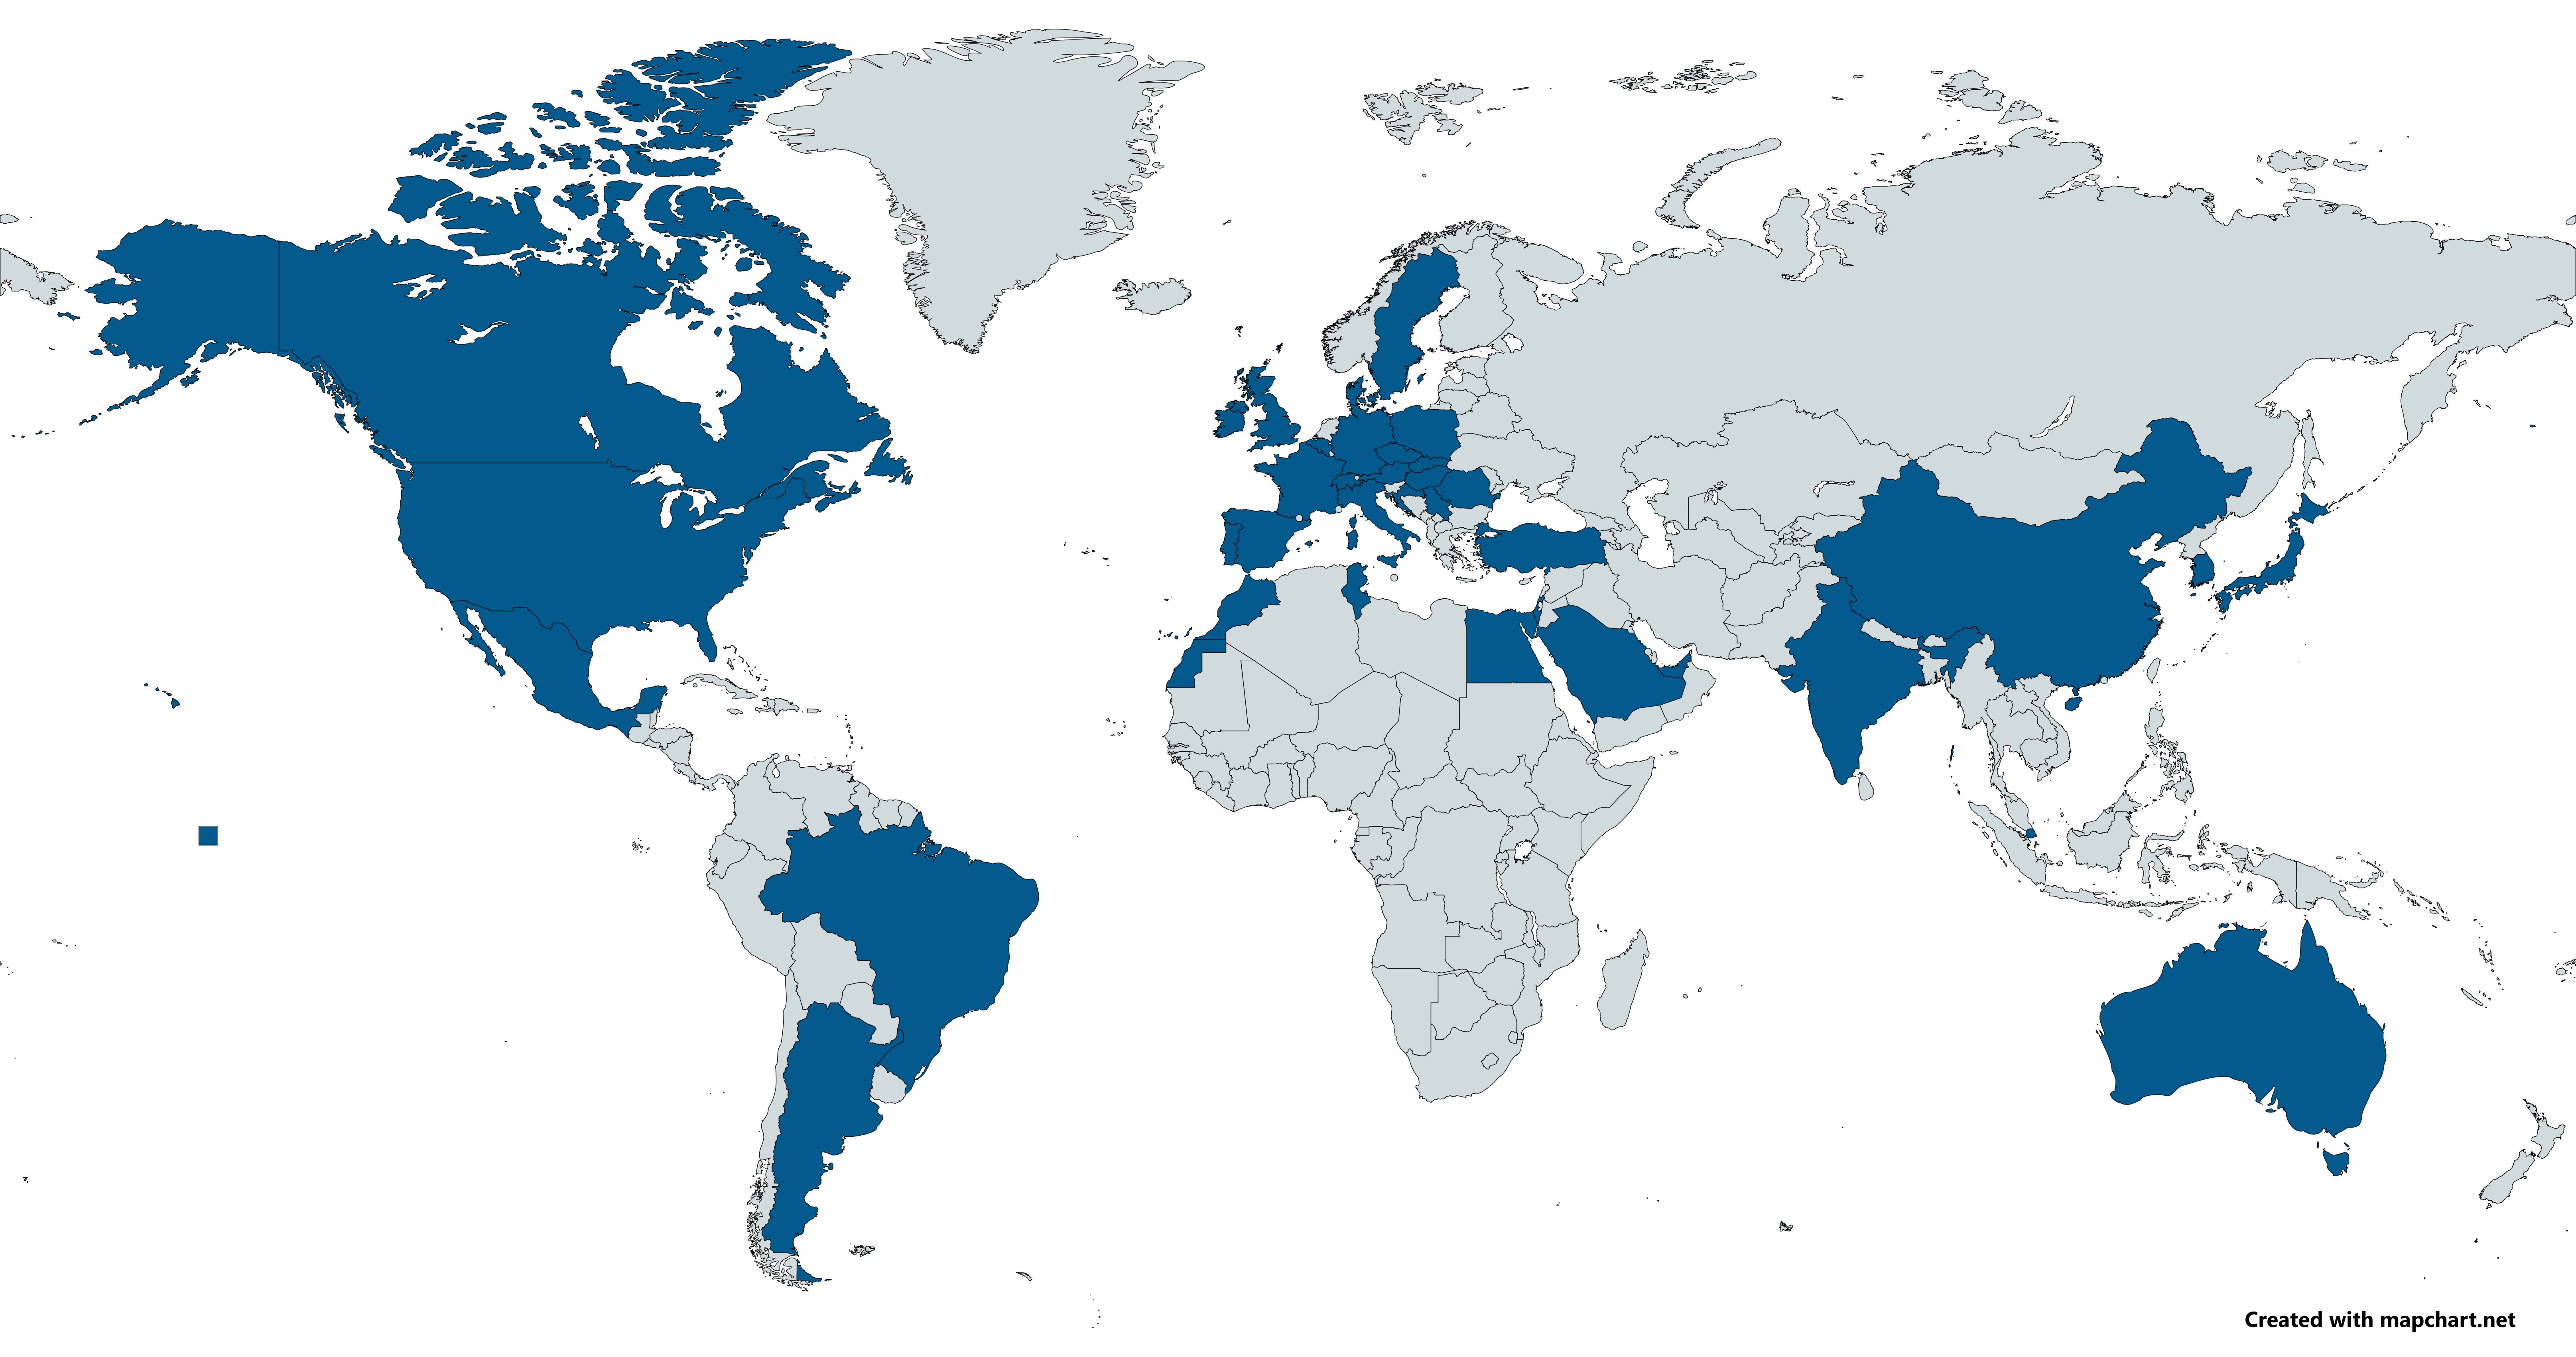
\includegraphics[width=0.9\linewidth]{Figures/introduction/map.png}
    \caption{Implantation du Groupe Segula Technologies dans le monde}
    \label{fig:segula-worldwide}
\end{figure}

La \autoref{fig:segula-worldwide} illustre la présence mondiale de Segula Technologies avec ses implantations dans les régions suivantes:

\begin{table}[H]
    \caption{Implantations de Segula Technologies par région}
    \label{tab:implantations-regions}
    \centering
    \begin{tabularx}{\textwidth}{|>{\bfseries\centering\arraybackslash}p{3.5cm}|X|}
        \hline
        \mdseries{Région} & \centering\mdseries{Pays} \tabularnewline
        \hline
        Amériques & Argentine, Brésil, Canada, États-Unis, Mexique \\
        \hline
        Asie-Océanie & Australie, Chine, Corée du Sud, Inde, Japon, Singapour \\
        \hline
        Afrique – Moyen Orient & Arabie Saoudite, Égypte, Émirats arabes unis, Israël, Maroc, Tunisie, Turquie \\
        \hline
        Europe & Allemagne, Autriche, Belgique, Croatie, Danemark, Espagne, France, Hongrie, Irlande, Italie, Pologne, Portugal, République tchèque, Roumanie, Royaume-Uni, Serbie, Slovaquie, Suède, Suisse \\
        \hline
    \end{tabularx}
\end{table}

\subsubsection*{Segula Technologies Maroc}

SEGULA Technologies Maroc est une filiale du groupe SEGULA Technologies en Afrique, créée en 2007. Grâce à ses bureaux d'études à Casablanca et à Agadir, ainsi sa filiale SIMRA. La filiale marocaine emploie plus de 700 ingénieurs et techniciens hautement qualifiés, avec un fort chiffre d'affaires plus de 22 millions d'euros en 2021. La filiale a travaillé sur la conception et l'industrialisation de nouveaux produits ou nouvelles usines pour ses clients. Elle offre des services d'ingénierie et de conseil pour la conception de véhicules, l'optimisation des processus de production, la gestion de la chaîne d'approvisionnement, l'analyse des coûts, la simulation et la modélisation.

\begin{figure}[H]
    \centering
    
\includegraphics[width=0.4\textwidth]{Figures/SIMRA.png}
    \caption{Logo de SIMRA - filiale de Segula Technologies Maroc}
    \label{fig:simra-logo}
\end{figure}

%% ---- I.2 Fiche technique ----
\subsection{Fiche technique}

Le \autoref{tab:fiche-technique} présente en détails l'ensemble des informations sur l'entreprise d'accueil :

\begin{table}[H]
    \caption{Fiche technique de Segula Technologies}
    \label{tab:fiche-technique}
    \centering
    \begin{tabularx}{\textwidth}{|>{\bfseries\raggedright}p{4.5cm}|X|}
        \hline
        \mdseries{Raison sociale} & SEGULA Technologies \\
        \hline
        \mdseries{Forme juridique} & Société par actions simplifiée \\
        \hline
        \mdseries{Année de création} & 1984 \\
        \hline
        \mdseries{Adresse postale} & 19 Rue d'Arras 92000 Nanterre, France \\
        \hline
        \mdseries{Activité} & Ingénierie, études techniques \\
        \hline
        \mdseries{Chiffre d'affaires (2023)} & 27 142 440 € \\
        \hline
        \mdseries{Implantations} & +140 implantations \\
        \hline
        \mdseries{Site web} & www.segulatechnologies.com/fr \\
        \hline
    \end{tabularx}
\end{table}

%% ---- I.3 Activités ----
\subsection{Activités}

Segula Technologies est le premier groupe européen de conseil et d'ingénierie en innovation technologique. Le groupe couvre toutes les phases du cycle de vie d'un projet, de sa définition (veille technologique, études de faisabilité technique, définition des stratégies, etc.) à sa concrétisation (conception, mise en œuvre et validation de solutions, etc.). L'activité s'organise autour de 2 axes :

\begin{itemize}
    \item[•] Conseil en technologie et en recherche \& développement.
    \item[•] Conseil en organisation et en systèmes d'information.
\end{itemize}

%% ---- I.4 Domaines d'intervention ----
\subsection{Domaines d'intervention}

Le groupe Segula Technologies travaille sur différents secteurs dont le secteur industriel et le secteur tertiaire. Au sein du secteur industriel, il joue un rôle très important en étant porté sur plusieurs domaines : l'automobile, l'aéronautique, le naval, le ferroviaire, l'énergie, et encore le pharmaceutique.

\begin{figure}[H]
    \centering
    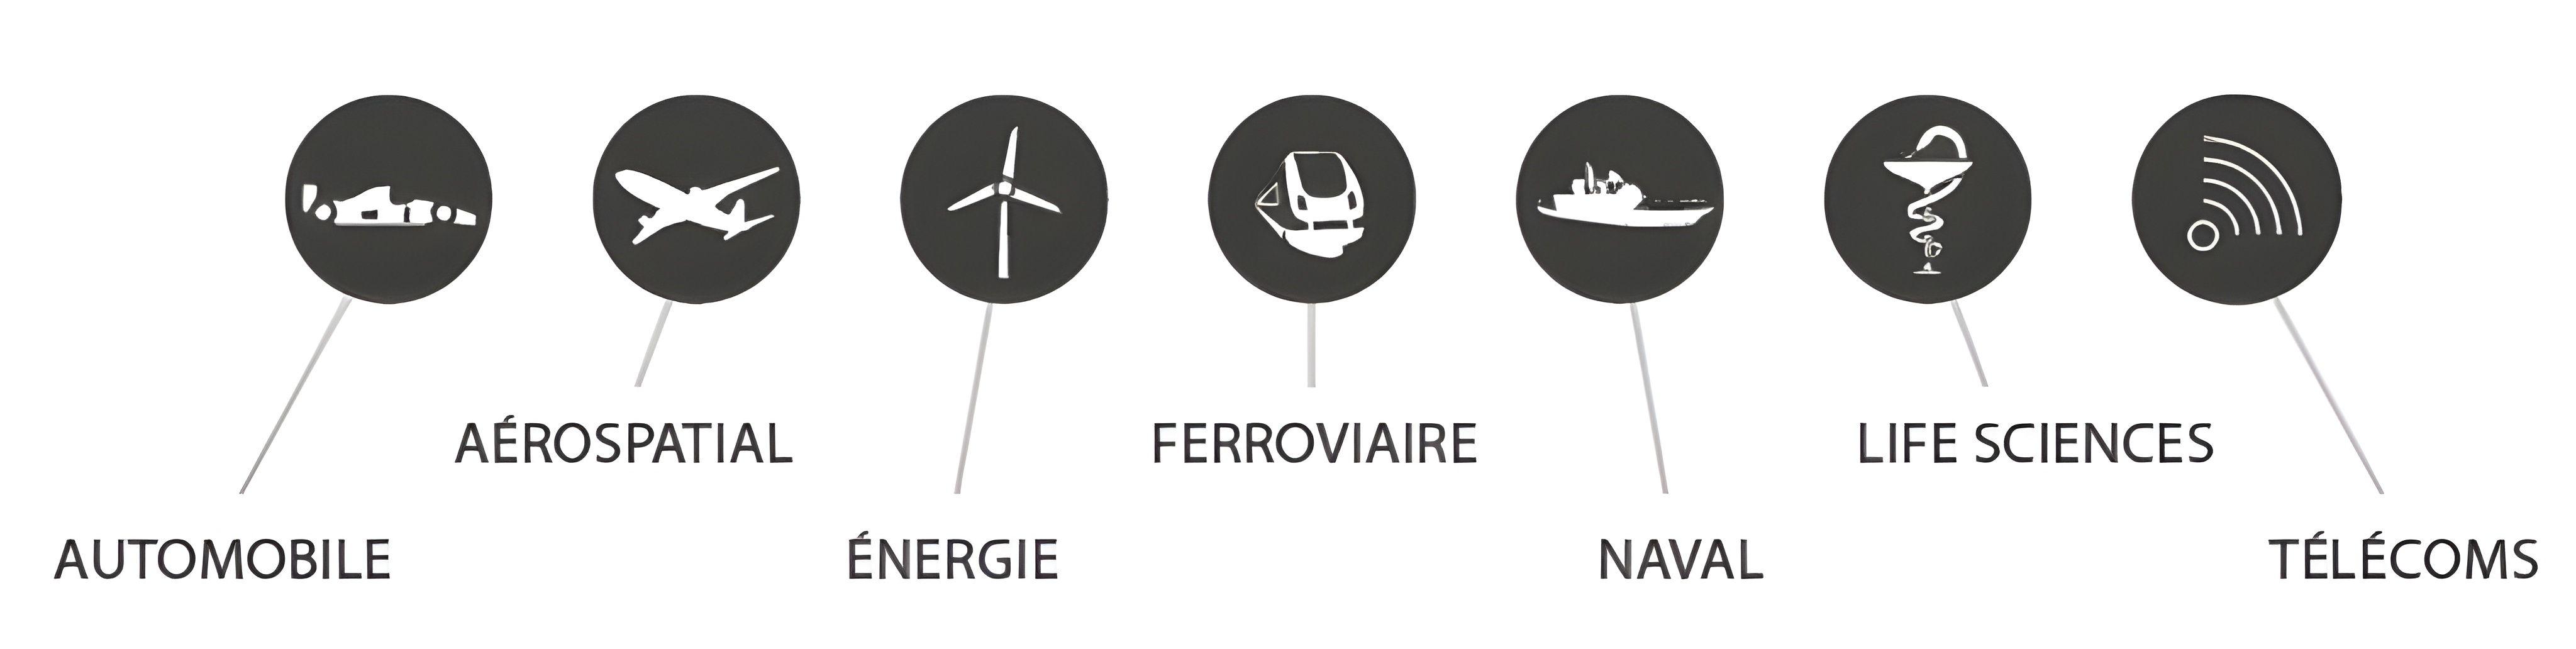
\includegraphics[width=0.9\linewidth]{Figures/introduction/domaines.png}
    \caption{Les divers secteurs d'activité de SEGULA Technologies}
\end{figure}

%% ---- I.5 Clients ----
\subsection{Clients}

Segula Technologies travaille avec une diversité de clients dans plusieurs secteurs, notamment l'automobile, l'aéronautique et le ferroviaire. En aéronautique, elle collabore avec des leaders de l'industrie pour développer des technologies avancées et optimiser la production. Dans le ferroviaire, Segula soutient des entreprises majeures en offrant des solutions innovantes pour le transport sur rail.

Dans le secteur automobile, l'un des principaux clients de Segula Technologies est Stellantis né de la fusion entre PSA (Peugeot Société Anonyme) et FCA (Fiat Chrysler Automobiles), qui englobe les marques Peugeot, Citroën, DS, Opel et Vauxhall. En 2014, PSA détenait une part de marché de 11,8 \% en Europe, démontrant son influence et son importance dans l'industrie automobile.

Le \autoref{tab:clients-partenaires} présente les principaux clients et partenaires de Segula Technologies classés par secteur d'activité.

\begin{table}[H]
    \caption{Principaux clients et partenaires de Segula Technologies}
    \label{tab:clients-partenaires}
    \centering
    \renewcommand{\arraystretch}{1.8}
    \begin{tabularx}{\textwidth}{|>{\centering\arraybackslash}p{2.8cm}|X|}
        \hline
        \mdseries{Secteur} & \centering\mdseries{Clients / Partenaires} \tabularnewline
        \hline
        & \centering
          
\includegraphics[height=0.5cm]{Figures/logos-partners/cars/Stellantis.png} \hspace{0.3cm}
          
\includegraphics[height=0.5cm]{Figures/logos-partners/cars/Peugeot.png} \hspace{0.3cm}
          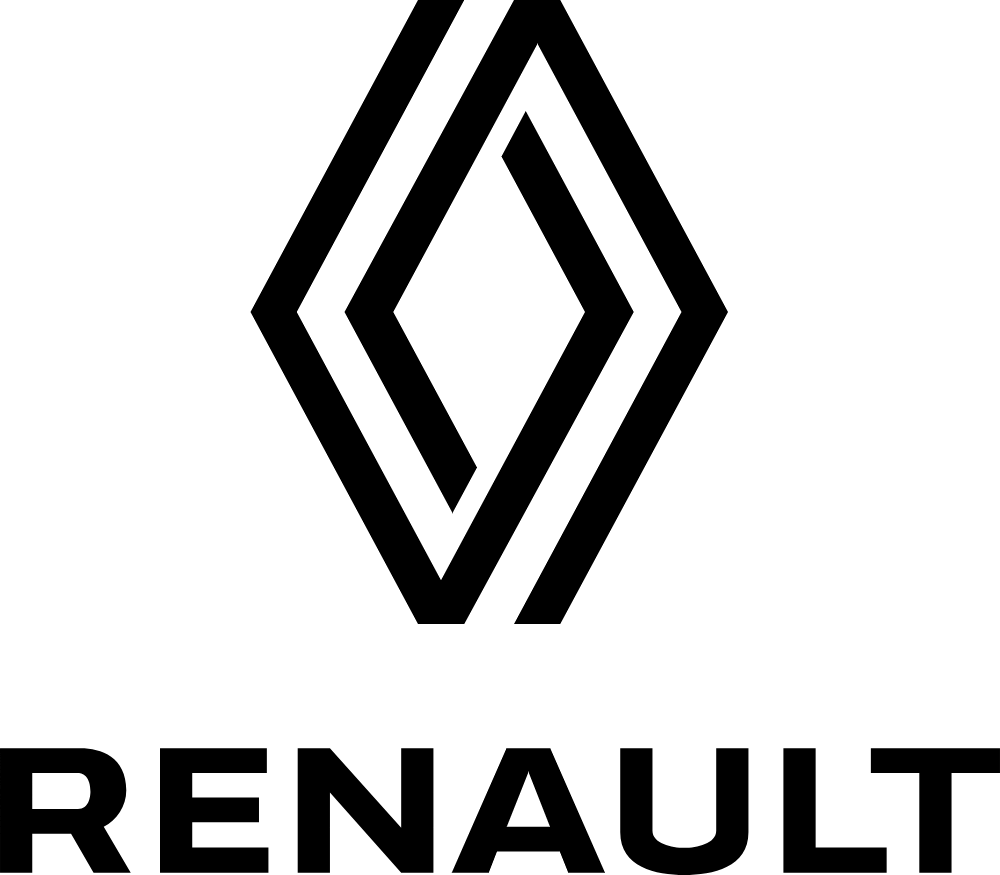
\includegraphics[height=0.5cm]{Figures/logos-partners/cars/Renault.png} \hspace{0.3cm}
          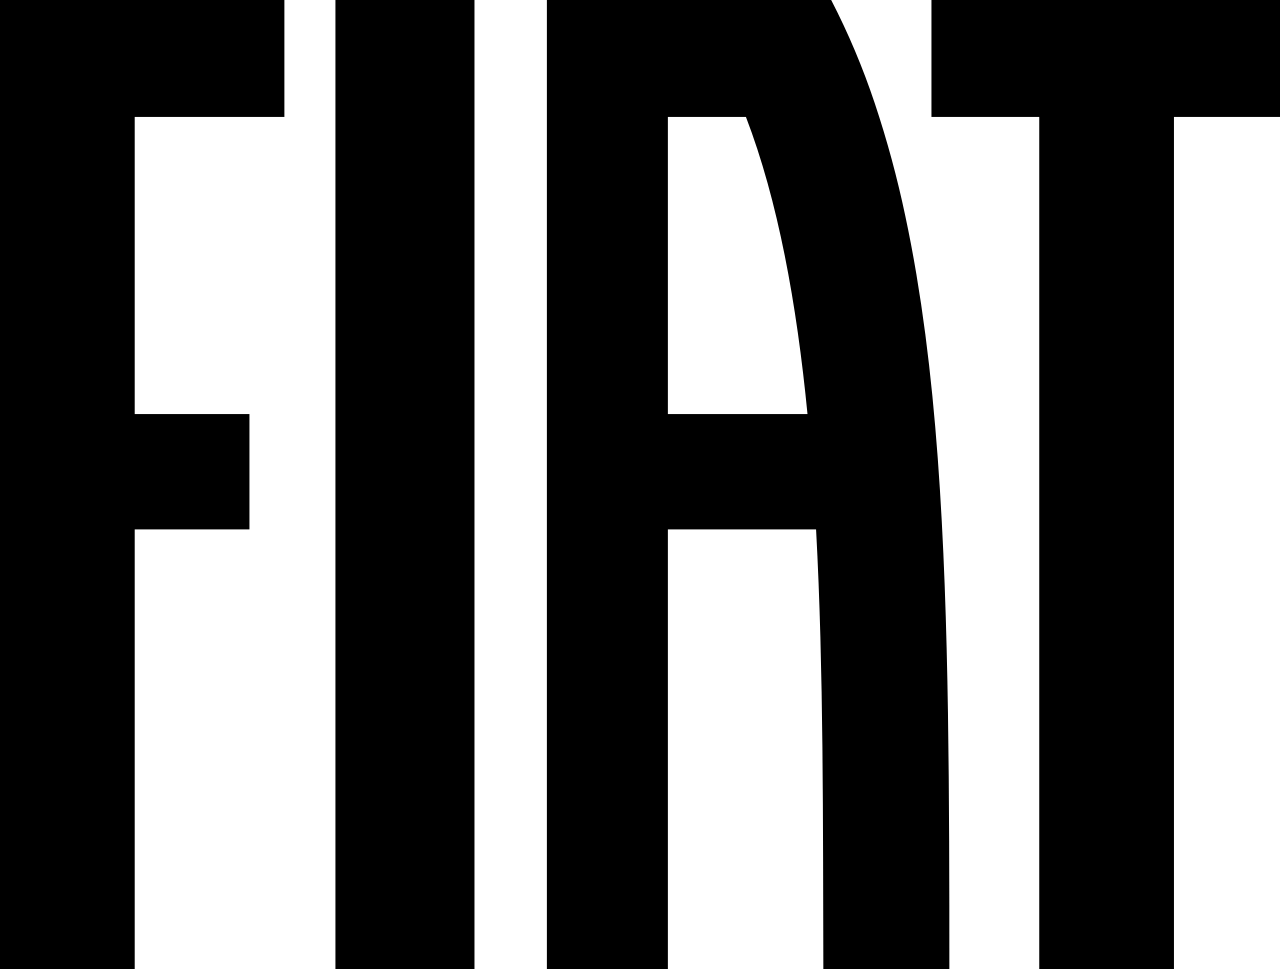
\includegraphics[height=0.5cm]{Figures/logos-partners/cars/FIAT.png} \tabularnewline
        \mdseries{Automobile}
        & \centering
          
\includegraphics[height=0.5cm]{Figures/logos-partners/cars/DS.png} \hspace{0.3cm}
          
\includegraphics[height=0.5cm]{Figures/logos-partners/cars/opel.png} \hspace{0.3cm}
          
\includegraphics[height=0.5cm]{Figures/logos-partners/cars/Dacia.png} \hspace{0.3cm}
          
\includegraphics[height=0.5cm]{Figures/logos-partners/cars/Continental.png} \tabularnewline
        & \centering
          
\includegraphics[height=0.5cm]{Figures/logos-partners/cars/gestamp.png} \hspace{0.3cm}
          
\includegraphics[height=0.5cm]{Figures/logos-partners/cars/Plastic_Omnium.png} \hspace{0.3cm}
          
\includegraphics[height=0.5cm]{Figures/logos-partners/cars/avtovaz.jpg} \hspace{0.3cm}
          
\includegraphics[height=0.5cm]{Figures/logos-partners/cars/smrc.jpg} \tabularnewline
        \hline
        \mdseries{Aéronautique}
        & \centering
          
\includegraphics[height=0.5cm]{Figures/logos-partners/aero/Airbus.png} \hspace{0.3cm}
          
\includegraphics[height=0.5cm]{Figures/logos-partners/aero/Safran.png} \hspace{0.3cm}
          
\includegraphics[height=0.5cm]{Figures/logos-partners/aero/Stelia.png} \tabularnewline
        \hline
        \mdseries{Ferroviaire}
        & \centering
          
\includegraphics[height=0.5cm]{Figures/logos-partners/ferroviaire/Alstom.png} \hspace{0.3cm}
          
\includegraphics[height=0.5cm]{Figures/logos-partners/ferroviaire/Intelligent Energy.png} \tabularnewline
        \hline
    \end{tabularx}
\end{table}

%%%%%%%%%%%%%%%%%%%%%%%%%%%%%%%%%%%%%%%%%%%%%%%%%%%%%%%%%%%
%%  SECTION II -- METHODOLOGIE DE TRAVAIL
%%%%%%%%%%%%%%%%%%%%%%%%%%%%%%%%%%%%%%%%%%%%%%%%%%%%%%%%%%%
\section{Méthodologie de travail}

\subsubsection{Choix de la démarche appropriée}

Pour garantir le succès de ce projet, il est essentiel de sélectionner une méthodologie de travail adaptée permettant de gérer et de structurer les différentes étapes, depuis la définition du problème jusqu'à son analyse, puis la mise en œuvre de solutions. Parmi les approches couramment utilisées pour la résolution de problèmes dans l'industrie figurent le DMAIC, le PDCA et la méthode 8D. Ces méthodes peuvent être catégorisées selon deux critères principaux :

\begin{itemize}
    \item La taille du problème à résoudre (petite, moyenne ou grande).
    \item La nature de la stratégie adoptée : s'il s'agit d'un processus d'amélioration continue ou de la résolution d'un problème spécifique.
\end{itemize}

À l'issue de cette analyse comparative, nous constatons que la démarche DMAIC est la plus adaptée à notre situation, compte tenu de la complexité du problème traité et de notre objectif d'amélioration à long terme.

\subsubsection{Définition de la démarche DMAIC}

DMAIC fait référence à un cycle visant à améliorer, optimiser et développer la conception au sein d'un service. Cette démarche est basée sur une approche structurée en cinq étapes ordonnancées selon une logique rigoureuse. Chaque lettre composant l'acronyme DMAIC correspond à l'initiale de la fonction de l'étape correspondante :

\begin{itemize}
    \item \mdseries{Define (Définir)} : consiste à définir clairement les objectifs du projet, les besoins des clients, les exigences et les contraintes.
    \item \mdseries{Measure (Mesurer)} : consiste à rassembler les informations nécessaires pour traiter le sujet de façon objective, ainsi qu'à identifier les zones critiques.
    \item \mdseries{Analyze (Analyser)} : vise à analyser les données collectées pour identifier les causes racines des problèmes et les opportunités d'amélioration.
    \item \mdseries{Improve (Améliorer/Innover)} : porte sur le développement et la mise en œuvre de solutions dont les performances correspondent aux objectifs fixés.
    \item \mdseries{Control (Contrôler/Vérifier)} : consiste à vérifier la performance et à suivre les résultats des solutions mises en œuvre afin de pérenniser les gains obtenus.
\end{itemize}

\subsubsection{Outils utilisés}

Pour mener à bien ce projet, plusieurs outils logiciels ont été mobilisés, chacun répondant à un besoin spécifique du cycle de développement.

\paragraph{Conception et développement.}

\begin{figure}[H]
\centering
\begin{minipage}[t]{0.45\textwidth}
    \centering
    
\includegraphics[height=1.8cm]{Figures/tools/catia.png}\\[0.6em]
    \mdseries{CATIA V5}\\
    \textit{Modélisation 3D des pièces\\et exécution des macros}
\end{minipage}
\hfill
\begin{minipage}[t]{0.45\textwidth}
    \centering
    
\includegraphics[height=1.8cm]{Figures/tools/vs.png}\\[0.6em]
    \mdseries{Visual Studio}\\
    \textit{Développement et débogage\\des macros VBA / CATScript}
\end{minipage}
\end{figure}

\paragraph{Analyse des données.}

\begin{figure}[H]
\centering
\begin{minipage}[t]{0.45\textwidth}
    \centering
    
\includegraphics[height=1.8cm]{Figures/tools/excel.png}\\[0.6em]
    \mdseries{Microsoft Excel}\\
    \textit{Manipulation des données\\et rapports de conformité}
\end{minipage}
\hfill
\begin{minipage}[t]{0.45\textwidth}
    \centering
    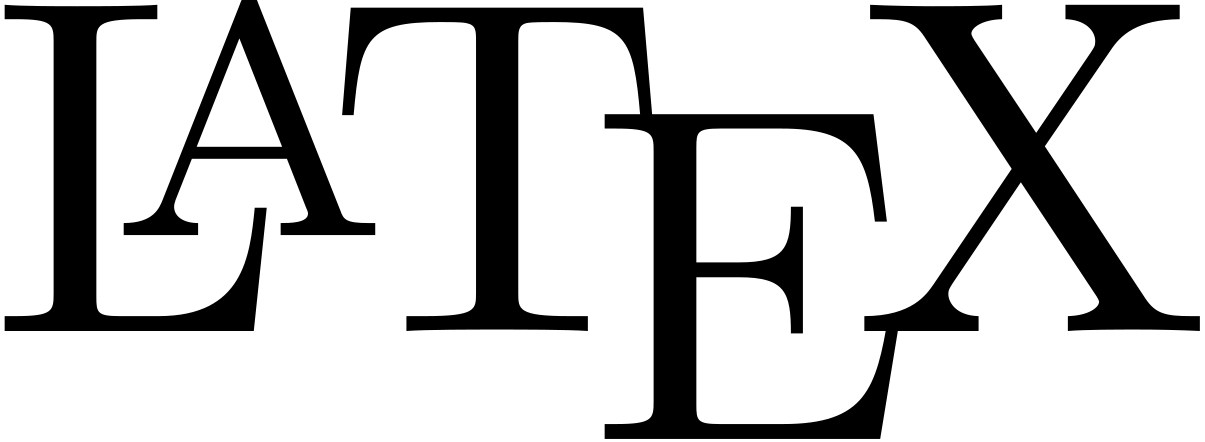
\includegraphics[height=1.8cm]{Figures/tools/latex.png}\\[0.6em]
    \mdseries{\LaTeX}\\
    \textit{Rédaction structurée du rapport\\avec gestion automatique des références}
\end{minipage}
\end{figure}

\chapter{Généralités sur l'industrie automobile}
\label{cp:generalites-automobile}

\textit{Ce deuxième chapitre vise à établir un socle de connaissances générales sur le secteur automobile, en abordant ses fondements historiques, ses évolutions technologiques et les grands enjeux auxquels il fait face aujourd'hui. Il permettra de situer le contexte industriel dans lequel s'inscrit ce projet, en mettant en lumière les principales étapes du cycle de développement d'un véhicule, les exigences réglementaires en matière de sécurité, ainsi que les approches numériques de plus en plus sollicitées pour anticiper et optimiser les performances des véhicules. Ces notions fondamentales serviront de base pour la compréhension des travaux réalisés dans la suite de ce rapport.}

\section{Classification des segments automobiles}

Dans l'industrie automobile, les véhicules sont classés par segments selon leurs dimensions, leur type d'utilisation et leur positionnement sur le marché. Cette classification permet aux constructeurs de cibler différents profils de clientèle et de structurer leur gamme de produits. Le \autoref{tab:segments-automobiles} présente les principaux segments utilisés en Europe.

\begin{table}[H]
    \caption{Classification des segments automobiles}
    \label{tab:segments-automobiles}
    \centering
    \small
    \renewcommand{\arraystretch}{1.4}
    \begin{tabularx}{\textwidth}{|>{\cellcolor{ensablue!15}\bfseries\centering\arraybackslash}p{1.8cm}|>{\centering\arraybackslash}X|>{\centering\arraybackslash}p{2.8cm}|>{\centering\arraybackslash}X|}
        \hline
        \rowcolor{ensablue!25}
        \textbf{Segment} & \textbf{Dénomination} & \textbf{Dimensions} & \textbf{Type d'utilisation} \\
        \hline
        B0 & Micro Urbaine & < 3,1 m & Zone urbaine -- courte distance \\
        \hline
        A & Urbaine & 3,1 m -- 3,6 m & Zone urbaine -- courte et moyenne distance \\
        \hline
        B & Citadine polyvalente & 3,6 m -- 4,1 m & Multi utilisations \\
        \hline
        B+ & Citadine monospace & 3,6 m -- 4,1 m & Multi utilisations \\
        \hline
        C & Compactes & 4,1 m -- 4,5 m & Familiale -- longues distances \\
        \hline
        D & Berlines & 4,5 m -- 4,8 m & Familiale confortable -- longue distance \\
        \hline
        E & Grandes routières & 4,9 m -- 5 m & Familiale confortable -- longue distance \\
        \hline
        F & Berlines de luxe & 5 m ou plus & Voiture luxueuse \\
        \hline
        SUV -- Crossover & Véhicule utilitaire sportif & 4,1 m -- 5 m & Familiale confortable -- longue distance -- parfois 4$\times$4 \\
        \hline
    \end{tabularx}
\end{table}

\chapter{Définir}
\label{cp:definir}

\textit{À compléter.}

\chapter{Mesurer}
\label{cp:mesurer}

Après avoir défini les objectifs et le périmètre du projet dans la phase \textit{Définir}, nous entamons désormais la phase \textit{Mesurer} de la démarche DMAIC. Cette étape consiste à quantifier l'état actuel du processus de vérification qualité, à identifier les critères de conformité critiques et à établir des indicateurs de performance mesurables.

L'objectif de cette phase est double : d'une part, collecter les données nécessaires pour évaluer l'ampleur du problème de contrôle qualité sur les surfaces CATIA, et d'autre part, formaliser les règles métier qui serviront de référence pour automatiser les vérifications. Nous nous concentrons en particulier sur les défauts surfaciques tels que les auto-intersections, qui constituent l'un des principaux obstacles à la fabricabilité des pièces conçues.

Cette partie présente les critères de qualité identifiés, leurs fondements mathématiques, ainsi que les mécanismes de détection que les macros Q-Checker métier devront automatiser.

\section{Convention de nommage}

\subsection{Contexte et enjeu}

Dans un environnement de conception collaboratif tel que CATIA~V5, chaque entité --- pièce (\textit{Part}), assemblage (\textit{Product}), surface ou feature --- est identifiée avant tout par son \textbf{nom} dans l'arbre de spécifications. Ce nom constitue la clé d'accès à l'objet pour les outils PDM/PLM (ENOVIA, Windchill), pour les scripts d'automatisation et pour l'ensemble des métiers aval (FAO, FEA, approvisionnement). Une convention de nommage est donc bien plus qu'une question d'esthétique : c'est un \textbf{contrat de lisibilité} entre tous les acteurs de la chaîne numérique.

Chez Segula Technologies, les projets automotive impliquent plusieurs centaines de pièces, développées en parallèle par des équipes réparties. En l'absence d'une règle de nommage imposée et vérifiée automatiquement, des dérives apparaissent inévitablement : noms génériques (\texttt{Part1}, \texttt{Body2}), noms en minuscules, ou noms sans code département. Ces incohérences se répercutent directement sur la chaîne de valeur.

\subsection{Justification métier}

L'absence ou le non-respect d'une convention de nommage génère des dysfonctionnements concrets à plusieurs niveaux de la chaîne de développement produit. Le \autoref{tab:impacts-nommage} synthétise les principaux impacts identifiés au cours de la phase Mesurer.

\begin{table}[H]
    \centering
    \caption{Impacts métier d'une convention de nommage non respectée}
    \label{tab:impacts-nommage}
    \begin{tabularx}{\textwidth}{|>{\bfseries\raggedright\arraybackslash}p{3.8cm}|X|}
        \hline
        \rowcolor{headerblue}
        \textcolor{white}{\textbf{Domaine impacté}} & \centering\textcolor{white}{\textbf{Conséquence opérationnelle}} \tabularnewline
        \hline
        \rowcolor{rowlight}
        Gestion de données produit (PDM/PLM) & Un nom non conforme ne remonte pas correctement dans les requêtes ENOVIA/Wind\-chill. La pièce devient introuvable dans les référentiels, générant des doublons et des risques de livraison d'une version obsolète. \\
        \hline
        \rowcolor{rowwhite}
        Assemblage & Un nom générique (\texttt{Part1}, \texttt{Body2}) rend impossible l'identification rapide d'une pièce dans un assemblage de plusieurs centaines de composants, multipliant les erreurs de substitution lors des échanges inter-équipes. \\
        \hline
        \rowcolor{rowlight}
        Automatisation Q-Checker & Les scripts de contrôle qui filtrent les pièces par code famille (ex.\ \texttt{MEC-*}, \texttt{STR-*}) échouent silencieusement si les noms ne respectent pas le format attendu. Le contrôle qualité automatisé devient inopérant sur ces pièces. \\
        \hline
        \rowcolor{rowwhite}
        Revues de conception & Un arbre de spécifications incohérent ralentit l'identification des responsabilités et des jalons de validation. Le temps perdu à identifier les pièces se répercute directement sur le planning projet. \\
        \hline
        \rowcolor{rowlight}
        Approvisionnement & Une référence non conforme rompt la traçabilité vers la nomenclature de fabrication (BOM). L'ERP ne reconnaît pas la référence, bloquant les commandes fournisseurs. \\
        \hline
    \end{tabularx}
\end{table}

\subsection{Règle de nommage retenue}

La convention adoptée pour ce projet suit le format \texttt{XXX-NNNN}, défini comme suit :

\begin{itemize}
    \item[•] \textbf{\texttt{XXX}} : exactement trois lettres majuscules, représentant le code famille ou département (\texttt{MEC} pour mécanique, \texttt{STR} pour structure, \texttt{ASS} pour assemblage, etc.).
    \item[•] \textbf{\texttt{-}} : un tiret séparateur obligatoire.
    \item[•] \textbf{\texttt{NNNN}} : trois ou quatre chiffres de séquencement, commençant à \texttt{001}.
\end{itemize}

\noindent\textbf{Exemples conformes :} \texttt{MEC-001}, \texttt{STR-0042}, \texttt{ASS-1234}.

\noindent\textbf{Exemples non conformes :} \texttt{mec-001} (minuscules), \texttt{MEC001} (tiret absent), \texttt{MEC-001A} (caractère supplémentaire non autorisé), \texttt{Part1} (nom générique CATIA par défaut).

\subsection{Typologies de non-conformités observées}

L'analyse des fichiers CAO reçus et des projets en cours a permis d'identifier quatre typologies récurrentes de non-conformité, synthétisées dans le \autoref{tab:typologies-nommage}.

\begin{table}[H]
    \centering
    \caption{Typologies de non-conformités de nommage observées}
    \label{tab:typologies-nommage}
    \begin{tabularx}{\textwidth}{|>{\bfseries\raggedright\arraybackslash}p{3.5cm}|p{3.5cm}|X|}
        \hline
        \rowcolor{headerblue}
        \textcolor{white}{\textbf{Type}} & \textcolor{white}{\textbf{Exemple}} & \centering\textcolor{white}{\textbf{Cause racine}} \tabularnewline
        \hline
        \rowcolor{rowlight}
        Nom CATIA par défaut & \texttt{Part1}, \texttt{Product2} & Pièce créée mais jamais renommée. Résultat habituel d'un travail intermédiaire non finalisé avant livraison. \\
        \hline
        \rowcolor{rowwhite}
        Casse incorrecte & \texttt{mec-001}, \texttt{Mec-001} & Absence de règle imposée dans les gabarits projet ou saisie manuelle non contrôlée. \\
        \hline
        \rowcolor{rowlight}
        Format non conforme & \texttt{MEC001}, \texttt{ME-01} & Raccourci informel pris par le concepteur (deux lettres au lieu de trois, tiret oublié). \\
        \hline
        \rowcolor{rowwhite}
        Caractères non autorisés & \texttt{MEC-001\_REV2}, \texttt{MEC-001A} & Ajout d'un indice de révision dans le nom --- pratique héritée de flux non-PLM qui contamine l'identifiant officiel. \\
        \hline
    \end{tabularx}
\end{table}

\subsection{Stratégies de correction}

La correction des non-conformités de nommage obéit à une logique de priorité selon leur impact PDM. Le \autoref{tab:correction-nommage} présente les actions correctives recommandées.

\begin{table}[H]
    \centering
    \caption{Stratégies de correction des non-conformités de nommage}
    \label{tab:correction-nommage}
    \begin{tabularx}{\textwidth}{|>{\bfseries\raggedright\arraybackslash}p{3.5cm}|X|>{\centering\arraybackslash}p{2.2cm}|}
        \hline
        \rowcolor{headerblue}
        \textcolor{white}{\textbf{Action corrective}} & \centering\textcolor{white}{\textbf{Description}} & \textcolor{white}{\textbf{Priorité}} \tabularnewline
        \hline
        \rowcolor{rowlight}
        Renommage manuel immédiat & Pour un faible nombre de pièces non conformes, le concepteur renomme directement dans l'arbre CATIA ou dans l'interface PDM en suivant le format \texttt{XXX-NNNN}. & Haute \\
        \hline
        \rowcolor{rowwhite}
        Mise à jour des gabarits & Intégrer la convention dans les \textit{templates} CATIA (\texttt{.CATPart}, \texttt{.CATProduct}) utilisés à la création de fichiers, afin que chaque nouveau fichier respecte d'emblée le format. & Haute \\
        \hline
        \rowcolor{rowlight}
        Règle de contrôle PDM & Configurer une règle de validation dans ENOVIA/Windchill qui bloque le \textit{check-in} d'un fichier au nom non conforme, faisant du PDM le dernier rempart contre les incohérences. & Moyenne \\
        \hline
        \rowcolor{rowwhite}
        Sensibilisation des équipes & Organiser une session de formation courte pour rappeler la règle de nommage, illustrée par des exemples d'impacts réels, afin de réduire les dérives à la source. & Basse \\
        \hline
    \end{tabularx}
\end{table}

\begin{block}[note]
L'automatisation de la vérification de ces règles --- via une macro Q-Checker dédiée --- sera présentée dans la phase \textit{Innover}. La phase \textit{Mesurer} se concentre ici sur la compréhension du problème et la qualification de son impact métier.
\end{block}

\iffalse
    \item[�] \textbf{Récupération du document actif :} la macro accède au document ouvert dans CATIA via \texttt{CATIA.ActiveDocument}.
    \item[�] \textbf{Identification du type de document :} distinction entre \texttt{PartDocument} (pièce) et \texttt{ProductDocument} (assemblage) à l'aide de \texttt{TypeName()}.
    \item[�] \textbf{Validation du nom (pièce) :} le nom de la pièce est extrait et comparé au pattern \texttt{\textasciicircum[A-Z]\{3\}-\textbackslash d\{3,4\}\$} via une expression régulière.
    \item[�] \textbf{Parcours récursif (assemblage) :} pour un assemblage, la macro inspecte récursivement chaque sous-produit et valide son \texttt{PartNumber}.
    \item[�] \textbf{Génération du rapport :} les noms non conformes sont collectés et affichés dans un message récapitulatif à l'utilisateur.
\fi

%% ============================================================
%%  VÉRIFICATION SOLIDE ET PLEIN
%% ============================================================
\section{Vérification qu'un Part est solide et plein}

\subsection{Définition et contexte}

Dans l'environnement CATIA~V5, un \textit{Part} est un fichier de conception (\texttt{.CATPart}) qui peut contenir deux types de géométrie :

\begin{itemize}
    \item[•] \textbf{La géométrie solide} --- créée dans le workbench \textit{Part Design}, stockée dans le \texttt{PartBody}. Elle représente un volume fermé, avec une masse et des propriétés mécaniques calculables.
    \item[•] \textbf{La géométrie surfacique} --- créée dans le workbench \textit{Generative Shape Design} (GSD), stockée dans des \texttt{HybridBody}. Elle ne définit pas de volume à elle seule.
\end{itemize}

Un Part est dit \textbf{solide et plein} lorsque son corps principal (\texttt{MainBody}) contient des features opérationnelles dont le résultat cumulé produit un \textbf{volume strictement positif}. Un volume nul signifie que les opérations booléennes (ajouts, soustractions) se sont intégralement annulées, ou qu'aucune feature solide n'a été créée.

\subsection{Justification métier}

La vérification du volume n'est pas une simple formalité géométrique. Elle répond à des exigences concrètes dans un contexte industriel, synthétisées dans le \autoref{tab:justif-volume}.

\begin{table}[H]
    \centering
    \caption{Justification métier de la vérification volumique}
    \label{tab:justif-volume}
    \begin{tabularx}{\textwidth}{|>{\bfseries\raggedright\arraybackslash}p{3.8cm}|X|}
        \hline
        \rowcolor{headerblue}
        \textcolor{white}{\textbf{Exigence}} & \centering\textcolor{white}{\textbf{Conséquence d'un volume nul ou invalide}} \tabularnewline
        \hline
        \rowcolor{rowlight}
        Fiabilité des analyses aval (CAE) & Toute simulation numérique (éléments finis, calcul thermique, mise en forme) requiert un solide fermé avec un volume défini. Un Part au volume nul génère des erreurs dans les solveurs, compromettant l'intégrité des résultats. \\
        \hline
        \rowcolor{rowwhite}
        Cohérence de la nomenclature et des calculs de masse & Dans un assemblage CATIA (\texttt{CATProduct}), la masse de chaque composant est calculée à partir de son volume et de la densité du matériau. Un Part sans volume valide fausse les calculs de masse totale, impactant les études d'équilibre, de centrage et de résistance structurelle. \\
        \hline
        \rowcolor{rowlight}
        Faisabilité fabrication & Un modèle destiné à la fabrication (usinage, fonderie, impression~3D) doit représenter un volume solide continu. Un volume nul empêche la génération correcte des trajectoires d'outil (FAO) et rend la pièce non-usinable numériquement. \\
        \hline
        \rowcolor{rowwhite}
        Automatisation et contrôle qualité & La vérification systématique du volume par macro permet de filtrer les modèles invalides \textbf{avant} leur intégration dans un assemblage ou leur transmission à un bureau de fabrication, évitant des erreurs coûteuses en phase tardive du projet. \\
        \hline
    \end{tabularx}
\end{table}

\subsection{Mécanisme de mesure dans CATIA}

\subsubsection{Le workbench SPAWorkbench (Space Analysis)}

CATIA~V5 expose un workbench dédié aux mesures géométriques avancées : le \textbf{Space Analysis Workbench} (\texttt{SPAWorkbench}), accessible par macro via la méthode \texttt{GetWorkbench("SPAWorkbench")} appliquée au document actif. Ce workbench met à disposition la méthode \texttt{GetMeasurable()}, qui accepte un objet géométrique (Body, Face, Surface) et retourne un objet \texttt{Measurable} exposant les propriétés physiques calculées. Le \autoref{tab:spa-props} résume les principales propriétés disponibles.

\begin{table}[H]
    \centering
    \caption{Propriétés de mesure exposées par le SPAWorkbench}
    \label{tab:spa-props}
    \begin{tabularx}{\textwidth}{|>{\ttfamily\raggedright\arraybackslash}p{3.5cm}|X|>{\centering\arraybackslash}p{2.5cm}|}
        \hline
        \rowcolor{headerblue}
        \normalfont\textcolor{white}{\textbf{Propriété}} & \centering\textcolor{white}{\textbf{Signification}} & \textcolor{white}{\textbf{Unité SI}} \tabularnewline
        \hline
        \rowcolor{rowlight}
        .Volume & Volume total du solide & m$^{3}$ \\
        \hline
        \rowcolor{rowwhite}
        .Area & Aire totale de la surface extérieure & m$^{2}$ \\
        \hline
        \rowcolor{rowlight}
        GetCOG() & Coordonnées du centre de gravité & m \\
        \hline
    \end{tabularx}
\end{table}

\begin{block}[note]
CATIA travaille en système SI interne (mètres). Les valeurs retournées par \texttt{SPAWorkbench} doivent être converties : volume $\times 10^{9}$ pour obtenir des mm$^{3}$, aire $\times 10^{6}$ pour obtenir des mm$^{2}$.
\end{block}

\subsubsection{Mécanisme de calcul interne}

Le moteur géométrique de CATIA, basé sur le noyau \textbf{CGM} (\textit{Convergent Geometry Modeler}), calcule le volume par intégration numérique sur la représentation B-Rep (\textit{Boundary Representation}) du solide. La représentation B-Rep décrit un solide par l'ensemble de ses faces, arêtes et sommets. Pour qu'un volume soit calculable, trois conditions doivent être satisfaites :

\begin{itemize}
    \item[•] La géométrie doit être \textbf{fermée} (pas de face manquante).
    \item[•] Les normales de toutes les faces doivent pointer vers l'\textbf{extérieur} du solide.
    \item[•] Aucune \textbf{auto-intersection} ne doit exister sur les faces ou les arêtes.
\end{itemize}

Si l'une de ces conditions est violée, CATIA retourne un volume nul ou lève une erreur.

\subsection{Stratégies de correction}

Lorsque la macro détecte un volume nul ou une anomalie, plusieurs causes sont possibles. Le \autoref{tab:correction-volume} présente les cas fréquents et les actions correctives recommandées.

\begin{table}[H]
    \centering
    \caption{Stratégies de correction en cas de volume nul ou invalide}
    \label{tab:correction-volume}
    \begin{tabularx}{\textwidth}{|>{\bfseries\raggedright\arraybackslash}p{3.2cm}|p{3.8cm}|X|}
        \hline
        \rowcolor{headerblue}
        \textcolor{white}{\textbf{Cas détecté}} & \textcolor{white}{\textbf{Cause probable}} & \centering\textcolor{white}{\textbf{Action corrective}} \tabularnewline
        \hline
        \rowcolor{rowlight}
        PartBody vide & Aucune feature solide créée & Créer un Pad, Shaft ou autre feature de base dans Part Design. \\
        \hline
        \rowcolor{rowwhite}
        Volume = 0 avec features & Pocket de même dimension qu'un Pad (annulation totale) & Vérifier l'arbre de construction --- réduire la profondeur du Pocket. \\
        \hline
        \rowcolor{rowlight}
        Erreur de mesure & Géométrie invalide (auto-intersection, face ouverte) & Utiliser \textit{Analyze~$\rightarrow$ Check Geometry} pour localiser les défauts. \\
        \hline
        \rowcolor{rowwhite}
        Mauvais type de document & Fichier Product ou Drawing ouvert au lieu d'un Part & Ouvrir le fichier \texttt{.CATPart} correspondant. \\
        \hline
        \rowcolor{rowlight}
        Volume anormalement faible & Feature mal dimensionnée ou unités incorrectes & Vérifier les unités du document (\textit{Tools~$\rightarrow$ Options~$\rightarrow$ Parameters \& Measure}). \\
        \hline
    \end{tabularx}
\end{table}

\paragraph{Utiliser Check Geometry.}
L'outil \textbf{Analyze~$\rightarrow$ Check Geometry} (disponible dans Part Design et GSD) permet d'inspecter automatiquement un solide et d'identifier les faces en auto-intersection, les arêtes non-manifold (partagées par plus de deux faces) et les faces de surface nulle. Il est recommandé d'exécuter cet outil systématiquement avant toute analyse volumique par macro, afin de garantir la validité topologique du modèle.

\paragraph{Reconstruire l'arbre de features.}
Lorsqu'une annulation de volume est constatée, il est utile de \textbf{désactiver les features} une par une (clic droit $\rightarrow$ \textit{Deactivate}) pour identifier celle qui neutralise le volume. Cette approche par isolation permet un diagnostic rapide sans modifier définitivement la géométrie.

\subsection{Limites de la méthode}

\begin{itemize}
    \item[•] La macro analyse uniquement le \textbf{MainBody} (PartBody principal). Les corps secondaires (\textit{Bodies}) et les géométries surfaciques (\textit{HybridBodies}) ne sont pas pris en compte.
    \item[•] Le \texttt{SPAWorkbench} doit être disponible dans la licence CATIA active. En l'absence de ce module, la macro lèvera une erreur à l'appel de \texttt{GetWorkbench()}.
    \item[•] La précision du calcul volumique dépend de la tolérance de modélisation définie dans les options CATIA (\textit{Tools~$\rightarrow$ Options~$\rightarrow$ Shape~$\rightarrow$ General}).
\end{itemize}

\begin{block}[note]
L'implémentation de la macro de vérification volumique --- incluant le code VBA complet --- sera détaillée dans la phase \textit{Innover}. La présente section se limite à la compréhension du problème, à sa justification métier et aux stratégies de correction.
\end{block}

%% ============================================================
%%  AUTO-INTERSECTION
%% ============================================================
\section{Auto-intersection (Offset Clipping)}

%% --- Section 1 : Définition & fondements mathématiques ---
\subsection{Définition et fondements mathématiques}

L'\textbf{auto-intersection} (également appelée \textit{Offset Clipping}) est un défaut topologique qui survient lorsqu'une surface se croise elle-même dans l'espace 3D. Concrètement, deux zones distinctes de la surface viennent occuper la même position géométrique, créant une boucle de matière incohérente. Ce phénomène est couramment rencontré lors des opérations de création d'épaisseur (\textit{Thick Surface}) ou de décalage (\textit{Offset}) sur des géométries complexes telles que les congés serrés, les nervures fines ou les surfaces à forte courbure.

\paragraph{Rayon de courbure et surface décalée.}
Lors d'une opération d'\textit{Offset} ou de \textit{Thick Surface}, la surface décalée $S_d$ est obtenue en déplaçant chaque point de la surface d'origine le long de sa normale unitaire $\mathbf{n}$ :

\begin{equation*}
    S_d(u,v) = S(u,v) + d \cdot \mathbf{n}(u,v)
\end{equation*}

où $d$ est l'épaisseur (ou la distance de décalage). La validité géométrique de cette opération repose sur une condition simple : le \textbf{rayon de courbure minimal} $R_{\min}$ de la surface d'origine doit rester strictement supérieur à l'épaisseur appliquée :

\begin{equation*}
    \boxed{R_{\min} > d}
\end{equation*}

Physiquement, le rayon de courbure mesure le « degré de cambrage » local de la surface. Plus une zone est courbée, plus son rayon de courbure est petit. Lorsque l'épaisseur $d$ atteint ou dépasse $R_{\min}$, le point décalé franchit le centre de courbure : la normale s'inverse localement et la surface générée se replie sur elle-même. La topologie devient alors \textbf{Non-Manifold} --- c'est l'auto-intersection.

%% --- Section 2 : Condition d'auto-intersection ---
\subsection{Condition d'auto-intersection}

En termes simples, une surface présente une auto-intersection lorsque deux zones distinctes de cette surface se retrouvent au même endroit dans l'espace 3D. La surface « se traverse elle-même » en formant une \textbf{courbe d'auto-intersection}. Dans le cas courant du décalage, cette situation se produit précisément lorsque $d \ge R_{\min}$ : la surface décalée se croise dans les zones de forte courbure, comme illustré dans la \autoref{fig:self_intersection}.

\begin{figure}[hbt!]
    \centering
    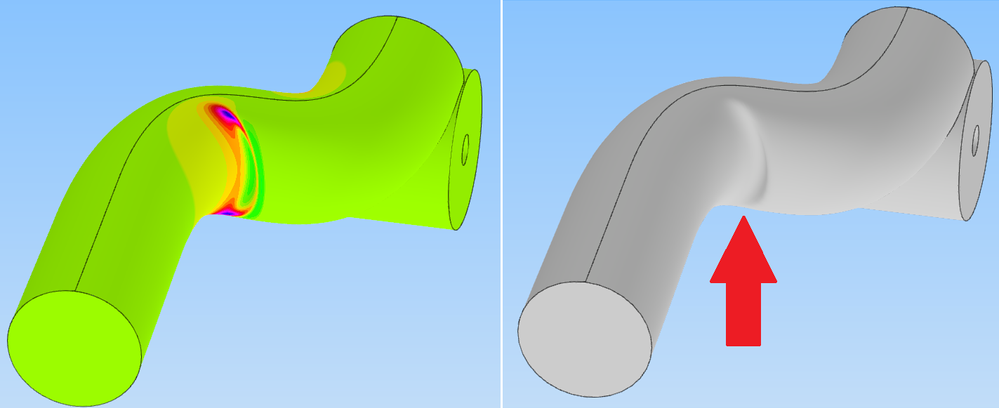
\includegraphics[width=0.45\textwidth]{Figures/self-intersection/self-intersection.png}
    \hfill
    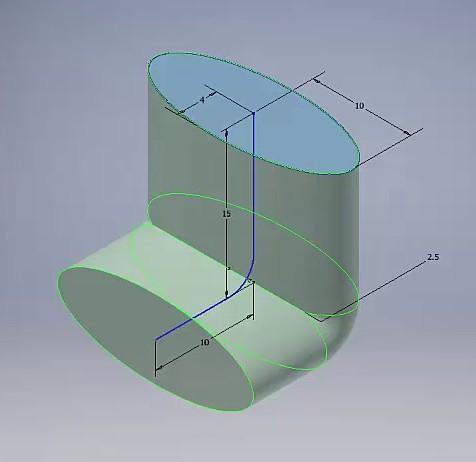
\includegraphics[width=0.45\textwidth]{Figures/self-intersection/self-intersection-2.jpg}
    \caption{Auto-intersection sur une surface décalée : la zone de forte courbure provoque un repliement de la surface sur elle-même.}
    \label{fig:self_intersection}
\end{figure}

%% --- Section 3 : Justification métier ---
\subsection{Justification métier}

Même lorsque CATIA parvient à générer la face décalée, celle-ci reste \textbf{techniquement inexploitable} par les métiers aval. La détection précoce de ce défaut est donc indispensable pour éviter des reprises coûteuses. Le \autoref{tab:impacts-auto-intersection} détaille les conséquences par domaine.

\begin{table}[H]
    \centering
    \caption{Conséquences industrielles de l'auto-intersection par domaine métier}
    \label{tab:impacts-auto-intersection}
    \begin{tabularx}{\textwidth}{|>{\bfseries\raggedright\arraybackslash}p{3.8cm}|X|}
        \hline
        \rowcolor{headerblue}
        \textcolor{white}{\textbf{Domaine}} & \centering\textcolor{white}{\textbf{Conséquence}} \tabularnewline
        \hline
        \rowcolor{rowlight}
        Fabrication assistée par ordinateur (FAO) & Les trajectoires d'outils CNC échouent ou génèrent des collisions face à une matière qui se croise elle-même. L'usinage devient imprévisible et potentiellement dangereux. \\
        \hline
        \rowcolor{rowwhite}
        Simulation par éléments finis (FEA) & Le maillage volumique ne peut pas être généré correctement sur une géométrie auto-intersectante : les éléments finis deviennent dégénérés, rendant les simulations invalides. \\
        \hline
        \rowcolor{rowlight}
        Injection plastique & Les contre-dépouilles créées par l'auto-intersection rendent le démoulage impossible sans modification de l'outillage. \\
        \hline
    \end{tabularx}
\end{table}

\begin{block}[note]
Dans l'industrie automobile, un défaut d'auto-intersection détecté tardivement --- après la livraison des outillages --- peut engendrer des coûts de reprise de plusieurs dizaines de milliers d'euros. D'où l'importance d'une détection automatisée dès la phase de conception.
\end{block}

%% --- Section 4 : Méthode de détection --- 
\subsection{Méthode de détection : la technique « Try-to-Join »}

L'API CATIA V5 ne fournit aucune fonction directe de type \texttt{Surface.IsSelfIntersecting()}. L'outil interactif \textit{Face Checker}, disponible dans le module \textit{Generative Shape Design}, permet certes de visualiser les auto-intersections, mais il n'est pas exposé dans l'API d'automatisation VBA/CATScript. Il est donc inutilisable dans une macro Q-Checker.

\paragraph{Principe de la technique.}
La solution retenue repose sur une approche indirecte baptisée \textbf{Try-to-Join}. L'idée est d'exploiter le fait que le noyau géométrique CGM de Dassault Systèmes effectue systématiquement un contrôle d'auto-intersection lors de toute opération topologique. Le principe se décompose en trois étapes :

\begin{enumerate}
    \item \textbf{Création d'un Join temporaire} --- La macro crée un objet \texttt{HybridShapeAssemble} (opération \textit{Join}) en prenant la surface cible comme unique entrée. Cette opération est ajoutée au \textit{HybridBody} du document.
    \item \textbf{Mise à jour forcée} --- L'appel à \texttt{Part.UpdateObject} déclenche le recalcul du Join par le noyau CGM. C'est à cette étape que le noyau effectue ses vérifications topologiques internes.
    \item \textbf{Capture du verdict} --- Si la surface est saine, le Join se calcule sans erreur. Si une auto-intersection est présente, le noyau CGM lève une exception que le bloc \texttt{On Error} de la macro intercepte. La surface est alors marquée comme défaillante.
\end{enumerate}

Cette technique transforme donc une \textbf{absence de fonction API} en un test fiable en s'appuyant sur les contrôles internes du noyau géométrique.

\paragraph{Avantages de l'approche.}
La technique Try-to-Join présente plusieurs atouts par rapport à une implémentation manuelle de détection :

\begin{itemize}
    \item[•] \textbf{Aucune dépendance externe :} elle utilise uniquement les objets natifs de CATIA, sans bibliothèque tierce.
    \item[•] \textbf{Fiabilité du noyau CGM :} le contrôle est délégué au même moteur géométrique que celui utilisé par les opérations de modélisation, garantissant une cohérence avec le comportement de CATIA.
    \item[•] \textbf{Simplicité d'implémentation :} quelques lignes de code VBA suffisent à mettre en place le test.
    \item[•] \textbf{Nettoyage automatique :} le Join temporaire est supprimé après le test, ne laissant aucune trace dans l'arbre de spécifications.
\end{itemize}

%% --- Section 5 : Pipeline CGM interne ---
\subsection{Pipeline interne du noyau CGM}

Pour mieux comprendre ce qui se passe « sous le capot » lors de l'appel à \texttt{Part.UpdateObject}, il est utile de décrire le pipeline de vérification exécuté par le noyau géométrique CGM (\textit{Convergence Geometric Modeler}) de Dassault Systèmes. Ce pipeline, résumé dans le \autoref{tab:etapes-cgm}, enchaîne six opérations successives allant de la discrétisation grossière jusqu'à la confirmation exacte de l'intersection.

\begin{table}[H]
    \centering
    \caption{Pipeline de vérification d'auto-intersection du noyau CGM (6 étapes)}
    \label{tab:etapes-cgm}
    \begin{tabularx}{\textwidth}{|>{\centering\arraybackslash}p{0.8cm}|>{\bfseries\raggedright\arraybackslash}p{3.2cm}|X|}
        \hline
        \rowcolor{headerblue}
        \textcolor{white}{\textbf{N°}} & \textcolor{white}{\textbf{Opération}} & \centering\textcolor{white}{\textbf{Description}} \tabularnewline
        \hline
        \rowcolor{rowlight}
        1 & Tessellation & La surface est découpée en un maillage de petits triangles. Cette approximation facettée permet de travailler avec des géométries plus simples pour les étapes suivantes. \\
        \hline
        \rowcolor{rowwhite}
        2 & Construction de l'arbre BVH & Chaque triangle est enfermé dans une boîte englobante alignée sur les axes (AABB). Ces boîtes sont organisées dans un arbre hiérarchique binaire (\textit{Bounding Volume Hierarchy}), ce qui permet de réduire la complexité des tests d'intersection de $O(n^2)$ à $O(n \log n)$. \\
        \hline
        \rowcolor{rowlight}
        3 & Test triangle--triangle & Pour chaque paire de triangles dont les boîtes englobantes se chevauchent, un test d'intersection géométrique exact est effectué. Ce test repose sur le calcul des plans supports des triangles et la vérification des intervalles de projection. \\
        \hline
        \rowcolor{rowwhite}
        4 & Filtrage des adjacences & Les paires de triangles qui partagent une arête ou un sommet sont automatiquement exclues : leur contact est un voisinage normal et non une intersection. Ce filtrage élimine les faux positifs liés à la connectivité du maillage. \\
        \hline
        \rowcolor{rowlight}
        5 & Raffinement exact & Lorsque des candidats à l'intersection subsistent après le filtrage, le noyau revient à la représentation mathématique exacte de la surface pour confirmer ou infirmer l'intersection avec une très haute précision (de l'ordre de $10^{-7}$~mm). \\
        \hline
        \rowcolor{rowwhite}
        6 & Signalement d'erreur & Si une intersection est confirmée, le noyau lève une erreur topologique. Cette erreur est propagée jusqu'à la couche VBA et capturée par le bloc \texttt{On Error} de la macro, permettant d'identifier la surface fautive. \\
        \hline
    \end{tabularx}
\end{table}

Ce pipeline illustre la stratégie « du grossier au fin » (\textit{coarse-to-fine}) adoptée par CGM : les premières étapes éliminent rapidement la majorité des zones saines grâce à des tests peu coûteux (boîtes englobantes), et seules les zones suspectes font l'objet d'un calcul exact. Cette approche garantit un bon compromis entre \textbf{performance} et \textbf{précision}.

%% --- Section 6 : Stratégies de correction ---
\subsection{Stratégies de correction}

Lorsqu'une auto-intersection est détectée par la macro, le concepteur doit intervenir sur la géométrie pour restaurer une topologie valide. Le choix de la stratégie dépend de la localisation du défaut, de la complexité de la surface et des contraintes fonctionnelles de la pièce. Le \autoref{tab:strategies-correction} présente les principales approches de correction utilisées en pratique.

\begin{table}[H]
    \centering
    \caption{Stratégies de correction d'une auto-intersection}
    \label{tab:strategies-correction}
    \begin{tabularx}{\textwidth}{|>{\bfseries\raggedright\arraybackslash}p{3.5cm}|X|>{\centering\arraybackslash}p{2.5cm}|}
        \hline
        \rowcolor{headerblue}
        \textcolor{white}{\textbf{Stratégie}} & \centering\textcolor{white}{\textbf{Description}} & \textcolor{white}{\textbf{Cas d'usage}} \tabularnewline
        \hline
        \rowcolor{rowlight}
        Augmentation du rayon de congé & Augmenter les rayons des congés (\textit{Fillets}) dans la zone de conflit afin de respecter la condition $R_{\min} > d$. C'est la correction la plus directe lorsque le défaut provient d'un congé trop serré par rapport à l'épaisseur. & Congés serrés \\
        \hline
        \rowcolor{rowwhite}
        Réduction de l'épaisseur locale & Diminuer la valeur de décalage $d$ dans la zone concernée, ou appliquer un offset variable si le cahier des charges le permet. & Épaisseur excessive \\
        \hline
        \rowcolor{rowlight}
        Healing / Lissage de courbure & Utiliser le \textit{Healing Assistant} ou l'outil \textit{Curve Smooth} de CATIA pour éliminer les micro-variations de courbure locales qui provoquent des pics de courbure sous le seuil $R_{\min}$. & Micro-défauts \\
        \hline
        \rowcolor{rowwhite}
        Découpe et reconstruction locale & Supprimer la zone de conflit et reconstruire la transition via un \textit{Multi-sections Surface}, un \textit{Blend} ou un \textit{Fill}. Cette approche offre un contrôle total sur la géométrie résultante. & Défauts localisés \\
        \hline
        \rowcolor{rowlight}
        Simplification géométrique & Remplacer une surface complexe (multi-congés, raccords G2) par une géométrie plus simple tout en respectant les tolérances fonctionnelles. & Géométries trop complexes \\
        \hline
    \end{tabularx}
\end{table}

En pratique, la correction suit une logique de \textbf{moindre modification} : on privilégie d'abord les ajustements paramétriques simples (augmentation de rayon, réduction d'épaisseur) avant de recourir à une reconstruction locale, plus lourde à mettre en œuvre et plus susceptible de modifier l'intention de conception.

%% --- Section 7 : Limites et perspectives ---
\subsection{Limites et perspectives}

\paragraph{Limites identifiées.}
Malgré son efficacité, la technique Try-to-Join présente plusieurs limites inhérentes au fonctionnement du noyau CGM et à l'environnement CATIA. Le \autoref{tab:limites-auto-intersection} en dresse la synthèse.

\begin{table}[H]
    \centering
    \caption{Limites de la détection automatisée de l'auto-intersection}
    \label{tab:limites-auto-intersection}
    \begin{tabularx}{\textwidth}{|>{\bfseries\raggedright\arraybackslash}p{3.8cm}|X|}
        \hline
        \rowcolor{headerblue}
        \textcolor{white}{\textbf{Limite}} & \centering\textcolor{white}{\textbf{Explication}} \tabularnewline
        \hline
        \rowcolor{rowlight}
        Faux négatifs & Si l'auto-intersection est d'amplitude inférieure à la tolérance interne du noyau CGM ($\approx 10^{-3}$~mm), le Join peut réussir sans détecter le défaut. La surface est alors validée à tort. \\
        \hline
        \rowcolor{rowwhite}
        Faux positifs & Une surface présentant des discontinuités de tangence marquées (raccords G0) peut faire échouer le Join sans être réellement auto-intersectante. Le défaut signalé est alors un problème de continuité, non d'auto-intersection. \\
        \hline
        \rowcolor{rowlight}
        Performance sur grands assemblages & Pour les assemblages volumineux comportant plus de 500 surfaces, la création et la suppression successives de Joins temporaires engendrent un temps de traitement significatif. \\
        \hline
        \rowcolor{rowwhite}
        Périmètre documentaire & La macro ne traite que les \texttt{CATPart}. Les documents de type \texttt{CATDrawing} et \texttt{CATAnalysis} ne sont pas pris en charge. \\
        \hline
        \rowcolor{rowlight}
        Absence de localisation précise & La technique indique \textit{qu'une} auto-intersection existe, mais ne fournit pas les coordonnées exactes de la zone de conflit. Le concepteur doit ensuite localiser visuellement le défaut. \\
        \hline
    \end{tabularx}
\end{table}

\paragraph{Perspectives d'amélioration.}
Plusieurs axes d'évolution sont envisageables pour renforcer l'outil de détection :

\begin{itemize}
    \item[•] \textbf{Coloration visuelle des défauts :} colorier automatiquement en rouge les surfaces défaillantes via \texttt{VisProperties.SetRealColor}, permettant au concepteur d'identifier instantanément les zones à corriger dans l'arbre de spécifications.
    \item[•] \textbf{Export du rapport en CSV :} générer un fichier de traçabilité contenant le nom de chaque surface, son statut (conforme / non conforme) et l'horodatage du contrôle, pour intégration dans le processus qualité du projet.
    \item[•] \textbf{Seuil de tolérance configurable :} permettre à l'utilisateur de définir la tolérance angulaire et positionnelle utilisée par le test, afin d'adapter la sensibilité de la détection au contexte métier (aéronautique vs.\ automobile, par exemple).
    \item[•] \textbf{Chaîne de contrôle intégrée :} chaîner la vérification d'auto-intersection avec les autres contrôles surfaciques (vrillage, \textit{sliver faces}, solidité) dans une macro unique, offrant un rapport qualité complet en une seule exécution.
    \item[•] \textbf{Migration vers 3DEXPERIENCE :} dans le cadre d'une future migration vers la plateforme 3DEXPERIENCE, explorer les nouvelles API de vérification géométrique qui pourraient offrir un accès direct aux fonctions de détection d'auto-intersection.
\end{itemize}

%% ============================================================
%%  VRILLAGE
%% ============================================================
\section{Vrillage (Auto-repliement)}

\subsection{Définition et fondements mathématiques}

Le vrillage (ou \textit{auto-repliement}) est une anomalie topologique majeure survenant lors de la génération de surfaces complexes via les fonctions de balayage (\textit{Sweep}) ou de surfaces multi-sections. Il se traduit par une inversion locale de la matière où la surface se croise elle-même.

Pour qu'une surface $\mathbf{S}(u,v)$ soit valide, sa paramétrisation doit être régulière. Le déterminant du Jacobien ($J$) traduit cette régularité :
\begin{equation*}
    J(u,v) = \left\| \frac{\partial \mathbf{S}}{\partial u} \times \frac{\partial \mathbf{S}}{\partial v} \right\|
\end{equation*}

\begin{itemize}
    \item[�] \textbf{Surface saine :} $J(u,v) > 0$ sur l'ensemble du domaine paramétrique.
    \item[�] \textbf{Vrillage :} apparaît lorsque $J(u,v) \le 0$. La surface perd alors sa propriété de variété (\textit{manifold}) ; les vecteurs tangents deviennent colinéaires, provoquant un effondrement géométrique.
\end{itemize}

Trois causes racines génèrent ce défaut en CAO :
\begin{itemize}
    \item[�] \textbf{Défaut de couplage :} mauvaise correspondance des points de fermeture (\textit{Closing Points}) entre sections.
    \item[�] \textbf{Conflit de tangence :} vecteurs de tangence opposés aux extrémités forçant une boucle.
    \item[�] \textbf{Saturation de l'épine (\textit{Spine}) :} rayon de courbure de la courbe guide inférieur à la demi-largeur de la section balayée.
\end{itemize}

\subsection{Justification métier : pourquoi détecter ce défaut ?}

Le vrillage constitue un critère d'exclusion lors du \textit{Q-Checking} :

\begin{itemize}
    \item[�] \textbf{Maillage (FEA) :} les solveurs ne peuvent pas traiter des faces auto-pénétrantes, entraînant un échec de simulation.
    \item[�] \textbf{Usinage (FAO) :} les normales erronées provoquent des collisions d'outil ou des trajectoires impossibles.
    \item[�] \textbf{Qualité perçue (Class A) :} rupture brutale des lignes de reflet (zébras), inacceptable en carrosserie.
\end{itemize}

La macro de détection permet d'identifier ces zones critiques avant toute transmission aux métiers aval.

\subsection{Pseudocode de l'algorithme}

% TODO : Insérer ici la capture d'écran du pseudocode / code VBA
\begin{center}
    \textit{[Image du pseudocode de la macro vrillage à insérer]}
    % \includegraphics[width=\textwidth]{Figures/pseudocode-vrillage.png}
\end{center}

\subsection{Étapes de la macro}

\begin{itemize}
    \item[�] \textbf{Discrétisation :} balayage de la surface sur une grille de points $P_{i,j}$.
    \item[�] \textbf{Calcul des normales :} extraction du vecteur unitaire $\mathbf{n}_{i,j}$ en chaque point.
    \item[�] \textbf{Test d'inversion :} si $\mathbf{n}_{i,j} \cdot \mathbf{n}_{i+1,j} < 0$, une inversion de normale est détectée.
    \item[�] \textbf{Verdict :} la zone est identifiée comme \textit{Twisted Surface} et la validation du modèle est bloquée.
\end{itemize}

% TODO : Insérer ici l'illustration visuelle des étapes de la macro
\begin{center}
    \textit{[Illustration visuelle des étapes à insérer]}
    % \includegraphics[width=\textwidth]{Figures/etapes-macro-vrillage.png}
\end{center}

\subsection{Organigramme de la macro}

% TODO : Insérer ici le flowchart de la macro vrillage
\begin{center}
    \textit{[Organigramme (flowchart) de la macro à insérer]}
    % \includegraphics[width=0.8\textwidth]{Figures/flowchart-vrillage.png}
\end{center}



\chapter{Analyser}
\label{cp:analyser}

La phase \textbf{Analyser} constitue le cœur de la démarche DMAIC. Après avoir défini le problème et mesuré les données pertinentes, il s'agit désormais d'identifier les causes profondes des non-conformités observées. Cette étape repose sur une investigation rigoureuse et structurée, mobilisant des outils statistiques et graphiques afin de distinguer les causes réelles des simples symptômes. L'objectif est de comprendre \textit{pourquoi} les écarts se produisent, avant toute tentative de correction ou d'amélioration.

Dans ce chapitre, nous mettons en œuvre plusieurs outils d'analyse causale appliqués aux données collectées sur le processus de fabrication étudié. Les résultats obtenus permettront d'orienter les actions d'amélioration présentées dans la phase suivante.

%------------------------------------------------------------------
\section{Analyse des causes racines des non-conformités}
\label{sec:analyse-causes-racines}

L'identification des causes racines est une étape essentielle pour garantir que les actions correctives menées s'attaquent aux origines réelles des défauts, et non à leurs manifestations superficielles. Plusieurs méthodes complémentaires sont employées à cet effet.

%------------------------------------------------------------------
\subsection{Diagramme ISHIKAWA}
\label{subsec:ishikawa}

Le diagramme d'Ishikawa, également appelé diagramme de cause-à-effet ou \textit{diagramme en arêtes de poisson}, est un outil visuel permettant de recenser et d'organiser l'ensemble des causes potentielles d'un effet indésirable. Développé par Kaoru Ishikawa dans les années 1960, il structure les causes selon les catégories classiques des \textbf{5M} : Matière, Milieu, Méthode, Machine et Main-d'œuvre.

Dans le contexte de notre étude, les catégories retenues ont été adaptées aux spécificités du processus de modélisation CATIA~V5. On distingue trois \textbf{causes techniques} --- Méthode, Géométrie et Logiciel --- et trois \textbf{causes opérationnelles} --- Utilisateur, Données~/~Fichier et Paramètres. L'effet ciblé regroupe les quatre types de défauts qualité identifiés sur les modèles CATIA~V5.

%--- Ishikawa colors (local) ---
\definecolor{ishitech}{HTML}{3D3B8E}
\definecolor{ishiops}{HTML}{0D6B53}
\definecolor{ishieff}{HTML}{6B1519}

\begin{figure}[htbp]
\centering
\vspace{1em}
\resizebox{\linewidth}{!}{%
\begin{tikzpicture}[
    >=stealth,
    font=\small,
    % Styles
    techcat/.style={
        rectangle, rounded corners=4pt,
        fill=ishitech, text=white,
        font=\small\bfseries, align=center,
        inner sep=5pt, minimum width=2.8cm, minimum height=0.7cm
    },
    opscat/.style={
        rectangle, rounded corners=4pt,
        fill=ishiops, text=white,
        font=\small\bfseries, align=center,
        inner sep=5pt, minimum width=2.8cm, minimum height=0.7cm
    },
    effectbox/.style={
        rectangle, rounded corners=5pt,
        fill=ishieff, text=white,
        font=\small\bfseries, align=center,
        inner sep=7pt, minimum width=3cm, minimum height=1.8cm
    },
    bone/.style={draw=gray!55, thin},
    causelabel/.style={font=\small, text=black, align=center},
    legendsq/.style={rectangle, minimum width=0.45cm, minimum height=0.38cm, inner sep=0pt},
]


%--- Spine ---%
\draw[gray!55, thick, ->] (0,0) -- (13.0,0);

%--- Effect box ---%
\node[effectbox] at (14.6, 0) {Défauts qualité\\[3pt]Modèle CATIA V5\\[3pt]4 types de défauts};

%--- Main diagonal bones ---
% Spine intersect points: x = 3.5, 7.5, 11.5
% Category centre x:      2.0, 6.0, 10.0   (shifted ~1.5 left of intersect)
% Category centre y: +4.2 (top) / -4.2 (bottom)

% Top bones
\draw[bone] (2.0, 4.2) -- (3.5, 0);
\draw[bone] (6.0, 4.2) -- (7.5, 0);
\draw[bone] (10.0, 4.2) -- (11.5, 0);

% Bottom bones
\draw[bone] (2.0, -4.2) -- (3.5, 0);
\draw[bone] (6.0, -4.2) -- (7.5, 0);
\draw[bone] (10.0, -4.2) -- (11.5, 0);

%--- Category boxes ---
\node[techcat] at (2.0,  4.85) {Méthode};
\node[techcat] at (6.0,  4.85) {Géométrie};
\node[techcat] at (10.0, 4.85) {Logiciel};

\node[opscat] at (2.0,  -4.85) {Utilisateur};
\node[opscat] at (6.0,  -4.85) {Données / Fichier};
\node[opscat] at (10.0, -4.85) {Paramètres};

%--- Sub-causes ---
% Parametric helper: bone from (x0,y0) to (x1,0)
%   P(t) = (x0 + t*(x1-x0),  y0*(1-t))

% == Méthode: (2.0, 4.2) -> (3.5, 0), dx=1.5, dy=-4.2 ==
% t=0.32 -> (2.48,  2.86)
\draw[bone] (2.48,  2.86) -- (1.0,  2.86);
\node[causelabel, anchor=east] at (0.95, 2.86) {Sketch non fermé};
% t=0.62 -> (2.93,  1.60)
\draw[bone] (2.93,  1.60) -- (1.5,  1.60);
\node[causelabel, anchor=east] at (1.45, 1.60) {Ordre des features};

% == Géométrie: (6.0, 4.2) -> (7.5, 0) — stubs LEFT ==
% t=0.28 -> (6.42, 3.02)
\draw[bone] (6.42,  3.02) -- (5.0,  3.02);
\node[causelabel, anchor=east] at (4.95, 3.02) {Flèche guide inv.};
% t=0.58 -> (6.87, 1.76)
\draw[bone] (6.87,  1.76) -- (5.4,  1.76);
\node[causelabel, anchor=east] at (5.35, 1.76) {Face manquante};

% == Logiciel: (10.0, 4.2) -> (11.5, 0) — stubs LEFT ==
% t=0.40 -> (10.60, 2.52)
\draw[bone] (10.60, 2.52) -- (9.1,  2.52);
\node[causelabel, anchor=east] at (9.05, 2.52) {Version CATIA};
% t=0.70 -> (11.05, 1.26)
\draw[bone] (11.05, 1.26) -- (9.55, 1.26);
\node[causelabel, anchor=east] at (9.50, 1.26) {Licence SPA abs.};

% == Utilisateur: (2.0, -4.2) -> (3.5, 0) ==
% t=0.32 -> (2.48, -2.86)
\draw[bone] (2.48, -2.86) -- (1.0, -2.86);
\node[causelabel, anchor=east] at (0.95, -2.86) {Feature désactivée};
% t=0.62 -> (2.93, -1.60)
\draw[bone] (2.93, -1.60) -- (1.5, -1.60);
\node[causelabel, anchor=east] at (1.45, -1.60) {Nommage arbitraire};

% == Données/Fichier: (6.0, -4.2) -> (7.5, 0) — stubs LEFT ==
% t=0.28 -> (6.42, -3.02)
\draw[bone] (6.42, -3.02) -- (5.0, -3.02);
\node[causelabel, anchor=east] at (4.95, -3.02) {Doc non valide};
% t=0.58 -> (6.87, -1.76)
\draw[bone] (6.87, -1.76) -- (5.4, -1.76);
\node[causelabel, anchor=east] at (5.35, -1.76) {PartBody vide};

% == Paramètres: (10.0, -4.2) -> (11.5, 0) — stubs LEFT ==
% t=0.40 -> (10.60, -2.52)
\draw[bone] (10.60, -2.52) -- (9.1,  -2.52);
\node[causelabel, anchor=east] at (9.05, -2.52) {Offset excessif};
% t=0.70 -> (11.05, -1.26)
\draw[bone] (11.05, -1.26) -- (9.55, -1.26);
\node[causelabel, anchor=east] at (9.50, -1.26) {Unités incorrectes};

%--- Legend ---
\node[legendsq, fill=ishitech] at (1.2, -6.2) {};
\node[anchor=west, font=\small] at (1.5, -6.2) {Causes techniques};

\node[legendsq, fill=ishiops]  at (6.2, -6.2) {};
\node[anchor=west, font=\small] at (6.5, -6.2) {Causes opérationnelles};

\node[legendsq, fill=ishieff]  at (12.0, -6.2) {};
\node[anchor=west, font=\small] at (12.3, -6.2) {Effet (4 défauts)};

\end{tikzpicture}%
}
\caption{Diagramme d'Ishikawa --- causes racines des défauts qualité du modèle CATIA~V5.}
\label{fig:ishikawa}
\end{figure}

%==================================================================
\section{Arbres des causes par type de défaut}
\label{sec:arbres-causes}
%==================================================================

\subsection{Arbre des causes par défaut qualité}
\label{subsec:arbre-causes}

Afin d'approfondir l'analyse, un arbre des causes est construit pour chaque type de défaut identifié. Cette représentation hiérarchique permet de relier l'effet observé à ses causes directes, puis de descendre vers les causes racines sous-jacentes. Le premier défaut étudié est le volume nul (\textit{Part non solide}), détecté automatiquement par la macro VBS développée dans la phase Mesurer.

%--- Fault-tree colors (local) ---
\definecolor{fteffect}{HTML}{6B1519}
\definecolor{ftdirect}{HTML}{7B4A00}
\definecolor{ftroot}{HTML}{3D3D3D}

\begin{figure}[htbp]
\centering
\vspace{0.5em}
\resizebox{\linewidth}{!}{%
\begin{tikzpicture}[
    node distance=0pt,
    font=\small,
    effectnode/.style={
        rectangle, rounded corners=6pt,
        fill=fteffect, text=white,
        font=\small\bfseries, align=center,
        inner sep=8pt, minimum width=5.5cm, minimum height=1.1cm
    },
    directnode/.style={
        rectangle, rounded corners=5pt,
        fill=ftdirect, text=white,
        font=\small\bfseries, align=center,
        inner sep=6pt, minimum width=3.8cm, minimum height=0.9cm
    },
    rootnode/.style={
        rectangle, rounded corners=4pt,
        fill=ftroot, text=white,
        font=\small, align=center,
        inner sep=5pt, minimum width=3.5cm, minimum height=0.75cm
    },
    conn/.style={draw=gray!60, thin},
]

% ============================================================
% Draw ALL lines first — nodes are painted on top afterwards
% Node geometry (minimum heights in cm = abstract units here):
%   effectnode h=1.1  → south at y = -0.55
%   directnode h=0.9  → south at y_center - 0.45
%   rootnode   h=0.75 → north at y_center + 0.375, south at y_center - 0.375
%
%   d1/d2/d3 at y=-3.2  → south = -3.65
%   r*a at y=-5.0  → north=-4.625, south=-5.375
%   r*b at y=-6.2  → north=-5.825, south=-6.575
%   r*c at y=-7.4  → north=-7.025
% ============================================================

% Effect -> horizontal bus
\draw[conn] (9, -0.55) -- (9, -1.1);
\draw[conn] (2, -1.1) -- (16, -1.1);

% Bus -> top of each direct-cause box
\draw[conn] (2,  -1.1) -- (2,  -2.75);
\draw[conn] (9,  -1.1) -- (9,  -2.75);
\draw[conn] (16, -1.1) -- (16, -2.75);

% Vertical trunks: direct-cause bottom -> below last root
\draw[conn] (2,  -3.65) -- (2,  -7.025);
\draw[conn] (9,  -3.65) -- (9,  -7.025);
\draw[conn] (16, -3.65) -- (16, -7.025);

% ============================================================
% Now draw all nodes ON TOP of the lines
% ============================================================

%--- Effect ---
\node[effectnode] at (9, 0) {Part non solide / Volume nul\\[2pt]{\footnotesize Détecté par la macro VBS}};

%--- Direct causes ---
\node[directnode] at (2,  -3.2) {PartBody vide};
\node[directnode] at (9,  -3.2) {Géométrie invalide};
\node[directnode] at (16, -3.2) {Document invalide};

%--- Root causes – PartBody vide ---
\node[rootnode] at (2, -5.0) {Aucune feature créée};
\node[rootnode] at (2, -6.2) {Features désactivées};
\node[rootnode] at (2, -7.4) {Annulation Pad-Pocket};

%--- Root causes – Géométrie invalide ---
\node[rootnode] at (9, -5.0) {Auto-intersection};
\node[rootnode] at (9, -6.2) {Face manquante};
\node[rootnode] at (9, -7.4) {Profil sketch ouvert};

%--- Root causes – Document invalide ---
\node[rootnode] at (16, -5.0) {Mauvais type de doc};
\node[rootnode] at (16, -6.2) {Licence SPA absente};
\node[rootnode] at (16, -7.4) {Unités incorrectes};

%--- Side labels ---
\node[font=\footnotesize\itshape, text=gray, anchor=east, align=center] at (-0.2,  0)    {Effet};
\node[font=\footnotesize\itshape, text=gray, anchor=east, align=center] at (-0.2, -3.2)  {Causes\\directes};
\node[font=\footnotesize\itshape, text=gray, anchor=east, align=center] at (-0.2, -6.2)  {Causes\\racines};

\end{tikzpicture}%
}
\caption{Arbre des causes --- défaut \textit{Part non solide / Volume nul}.}
\label{fig:arbre-causes-volume-nul}
\end{figure}

%------------------------------------------------------------------
\subsection{Surface auto-intersectante}
\label{subsec:arbre-auto-intersection}

Le deuxième défaut analysé est la \textbf{surface auto-intersectante}, caractéristique des défauts géométriques détectés dans le module GSD (Generative Shape Design) de CATIA~V5. Ce type de défaut survient lorsque la surface générée se recoupe elle-même, rendant la géométrie inexploitable pour les opérations aval. L'arbre des causes ci-dessous identifie trois familles de causes directes : le profil source, l'opération de surface et les paramètres de construction.

\definecolor{fteff2}{HTML}{6B1519}
\definecolor{ftdir2}{HTML}{7B4A00}

\begin{figure}[htbp]
\centering
\vspace{0.5em}
\resizebox{\linewidth}{!}{%
\begin{tikzpicture}[
    font=\small,
    effectnode/.style={rectangle, rounded corners=6pt, fill=fteff2, text=white,
        font=\small\bfseries, align=center, inner sep=8pt,
        minimum width=5.5cm, minimum height=1.1cm},
    directnode/.style={rectangle, rounded corners=5pt, fill=ftdir2, text=white,
        font=\small\bfseries, align=center, inner sep=6pt,
        minimum width=3.8cm, minimum height=0.9cm},
    rootnode/.style={rectangle, rounded corners=4pt, fill=ftroot, text=white,
        font=\small, align=center, inner sep=5pt,
        minimum width=3.5cm, minimum height=0.75cm},
    conn/.style={draw=gray!60, thin},
]
% --- Lines first ---
\draw[conn] (9,-0.55) -- (9,-1.1);
\draw[conn] (2,-1.1) -- (16,-1.1);
\draw[conn] (2,-1.1)  -- (2,-2.75);
\draw[conn] (9,-1.1)  -- (9,-2.75);
\draw[conn] (16,-1.1) -- (16,-2.75);
\draw[conn] (2,-3.65)  -- (2,-7.025);
\draw[conn] (9,-3.65)  -- (9,-7.025);
\draw[conn] (16,-3.65) -- (16,-7.025);
% --- Nodes ---
\node[effectnode] at (9,0) {Surface auto-intersectante\\[2pt]{\footnotesize Défaut géométrique --- GSD}};
\node[directnode] at (2,-3.2)  {Profil source};
\node[directnode] at (9,-3.2)  {Opération surface};
\node[directnode] at (16,-3.2) {Paramètres};
\node[rootnode] at (2,-5.0)  {Sketch ouvert ou croisé};
\node[rootnode] at (2,-6.2)  {Profil trop large};
\node[rootnode] at (2,-7.4)  {Contour self-croisé};
\node[rootnode] at (9,-5.0)  {Rayon guide trop faible};
\node[rootnode] at (9,-6.2)  {Offset excessif};
\node[rootnode] at (9,-7.4)  {Flèche guide inversée};
\node[rootnode] at (16,-5.0) {Tolérance trop élevée};
\node[rootnode] at (16,-6.2) {Loi de guide absente};
\node[rootnode] at (16,-7.4) {Accrochage manquant};
% --- Side labels ---
\node[font=\footnotesize\itshape, text=gray, anchor=east, align=center] at (-0.2,0)    {Effet};
\node[font=\footnotesize\itshape, text=gray, anchor=east, align=center] at (-0.2,-3.2) {Causes\\directes};
\node[font=\footnotesize\itshape, text=gray, anchor=east, align=center] at (-0.2,-6.2) {Causes\\racines};
\end{tikzpicture}%
}
\caption{Arbre des causes --- défaut \textit{Surface auto-intersectante}.}
\label{fig:arbre-causes-auto-intersection}
\end{figure}

%------------------------------------------------------------------
\subsection{Surface vrillée}
\label{subsec:arbre-surface-vrillee}

La \textbf{surface vrillée} (\textit{twisted}) constitue le troisième défaut étudié. Il s'agit d'un défaut d'orientation propre aux opérations Sweep et Loft du module GSD : la surface se tord le long de la trajectoire guide, produisant une géométrie incorrecte. Les causes sont regroupées en trois catégories — orientation des courbes, géométrie du guide, et paramétrage de l'opération.

\definecolor{fteff3}{HTML}{5C3A00}
\definecolor{ftdir3}{HTML}{1F3E6E}

\begin{figure}[htbp]
\centering
\vspace{0.5em}
\resizebox{\linewidth}{!}{%
\begin{tikzpicture}[
    font=\small,
    effectnode/.style={rectangle, rounded corners=6pt, fill=fteff3, text=white,
        font=\small\bfseries, align=center, inner sep=8pt,
        minimum width=5.5cm, minimum height=1.1cm},
    directnode/.style={rectangle, rounded corners=5pt, fill=ftdir3, text=white,
        font=\small\bfseries, align=center, inner sep=6pt,
        minimum width=3.8cm, minimum height=0.9cm},
    rootnode/.style={rectangle, rounded corners=4pt, fill=ftroot, text=white,
        font=\small, align=center, inner sep=5pt,
        minimum width=3.5cm, minimum height=0.75cm},
    conn/.style={draw=gray!60, thin},
]
% --- Lines first ---
\draw[conn] (9,-0.55) -- (9,-1.1);
\draw[conn] (2,-1.1) -- (16,-1.1);
\draw[conn] (2,-1.1)  -- (2,-2.75);
\draw[conn] (9,-1.1)  -- (9,-2.75);
\draw[conn] (16,-1.1) -- (16,-2.75);
\draw[conn] (2,-3.65)  -- (2,-7.025);
\draw[conn] (9,-3.65)  -- (9,-7.025);
\draw[conn] (16,-3.65) -- (16,-7.025);
% --- Nodes ---
\node[effectnode] at (9,0) {Surface vrillée (twisted)\\[2pt]{\footnotesize Défaut d'orientation --- GSD}};
\node[directnode] at (2,-3.2)  {Orientation courbes};
\node[directnode] at (9,-3.2)  {Géométrie guide};
\node[directnode] at (16,-3.2) {Opération Sweep/Loft};
\node[rootnode] at (2,-5.0)  {Flèches Loft inversées};
\node[rootnode] at (2,-6.2)  {Sens spline incohérent};
\node[rootnode] at (2,-7.4)  {Section mal orientée};
\node[rootnode] at (9,-5.0)  {Courbure excessive};
\node[rootnode] at (9,-6.2)  {Guide non continu};
\node[rootnode] at (9,-7.4)  {Points de passage faux};
\node[rootnode] at (16,-5.0) {Profil non normal guide};
\node[rootnode] at (16,-6.2) {Multi-section incomp.};
\node[rootnode] at (16,-7.4) {Loft mal défini};
% --- Side labels ---
\node[font=\footnotesize\itshape, text=gray, anchor=east, align=center] at (-0.2,0)    {Effet};
\node[font=\footnotesize\itshape, text=gray, anchor=east, align=center] at (-0.2,-3.2) {Causes\\directes};
\node[font=\footnotesize\itshape, text=gray, anchor=east, align=center] at (-0.2,-6.2) {Causes\\racines};
\end{tikzpicture}%
}
\caption{Arbre des causes --- défaut \textit{Surface vrillée}.}
\label{fig:arbre-causes-surface-vrillee}
\end{figure}

%------------------------------------------------------------------
\subsection{Non-conformité de nommage}
\label{subsec:arbre-nommage}

Le quatrième et dernier défaut traité concerne la \textbf{non-conformité de nommage} des données CATIA~V5. Bien qu'il n'entraîne pas de défaillance géométrique immédiate, un nommage arbitraire ou incohérent compromet la traçabilité, la maintenabilité et l'automatisation des traitements. Les causes sont articulées autour du nommage des features, des fichiers et des paramètres.

\definecolor{fteff4}{HTML}{3D3B8E}
\definecolor{ftdir4}{HTML}{0D5C47}

\begin{figure}[htbp]
\centering
\vspace{0.5em}
\resizebox{\linewidth}{!}{%
\begin{tikzpicture}[
    font=\small,
    effectnode/.style={rectangle, rounded corners=6pt, fill=fteff4, text=white,
        font=\small\bfseries, align=center, inner sep=8pt,
        minimum width=5.5cm, minimum height=1.1cm},
    directnode/.style={rectangle, rounded corners=5pt, fill=ftdir4, text=white,
        font=\small\bfseries, align=center, inner sep=6pt,
        minimum width=3.8cm, minimum height=0.9cm},
    rootnode/.style={rectangle, rounded corners=4pt, fill=ftroot, text=white,
        font=\small, align=center, inner sep=5pt,
        minimum width=3.5cm, minimum height=0.75cm},
    conn/.style={draw=gray!60, thin},
]
% --- Lines first ---
\draw[conn] (9,-0.55) -- (9,-1.1);
\draw[conn] (2,-1.1) -- (16,-1.1);
\draw[conn] (2,-1.1)  -- (2,-2.75);
\draw[conn] (9,-1.1)  -- (9,-2.75);
\draw[conn] (16,-1.1) -- (16,-2.75);
\draw[conn] (2,-3.65)  -- (2,-7.025);
\draw[conn] (9,-3.65)  -- (9,-7.025);
\draw[conn] (16,-3.65) -- (16,-7.025);
% --- Nodes ---
\node[effectnode] at (9,0) {Non-conformité nommage\\[2pt]{\footnotesize Défaut qualité données CATIA}};
\node[directnode] at (2,-3.2)  {Nommage features};
\node[directnode] at (9,-3.2)  {Nommage fichiers};
\node[directnode] at (16,-3.2) {Nommage paramètres};
\node[rootnode] at (2,-5.0)  {Noms par défaut (Pad.1)};
\node[rootnode] at (2,-6.2)  {Pas de préfixe standard};
\node[rootnode] at (2,-7.4)  {Langue incohérente};
\node[rootnode] at (9,-5.0)  {Nom générique (Part1)};
\node[rootnode] at (9,-6.2)  {Pas de numéro version};
\node[rootnode] at (9,-7.4)  {Extension incorrecte};
\node[rootnode] at (16,-5.0) {Valeur sans unité};
\node[rootnode] at (16,-6.2) {Nom non explicite};
\node[rootnode] at (16,-7.4) {Doublon de nom};
% --- Side labels ---
\node[font=\footnotesize\itshape, text=gray, anchor=east, align=center] at (-0.2,0)    {Effet};
\node[font=\footnotesize\itshape, text=gray, anchor=east, align=center] at (-0.2,-3.2) {Causes\\directes};
\node[font=\footnotesize\itshape, text=gray, anchor=east, align=center] at (-0.2,-6.2) {Causes\\racines};
\end{tikzpicture}%
}
\caption{Arbre des causes --- défaut \textit{Non-conformité de nommage}.}
\label{fig:arbre-causes-nommage}
\end{figure}

%==================================================================
\section{Convention de nommage}
\label{sec:naming-macro}
%==================================================================

%------------------------------------------------------------------
\subsection{Déroulement global de la macro}
\label{subsec:nm-deroulement}

% TODO : contenu à remplir --- texte descriptif et organigrammes à insérer ici.

%==================================================================
\section{Compréhension de la macro \texttt{silver\_faces.vbs}}
\label{sec:silver-faces-macro}
%==================================================================

%------------------------------------------------------------------
\subsection{Paramètres de configuration de la macro}
\label{subsec:sf-constantes}

La macro repose sur trois constantes dont les valeurs pilotent l'ensemble de la logique de détection et de correction :

\begin{table}[htbp]
\centering
\caption{Constantes de configuration de \texttt{silver\_faces.vbs}.}
\label{tab:sf-constantes}
\begin{tabularx}{\textwidth}{llX}
\toprule
\textbf{Constante} & \textbf{Valeur} & \textbf{Signification} \\
\midrule
SEUIL\_MM2    & \(0{,}01\ \text{mm}^2\)   & Toute surface dont l'aire est inférieure à ce seuil est considérée comme une silver face. \\
SEUIL\_DELETE & \(0{,}0001\ \text{mm}^2\) & En dessous de cette valeur, la surface est quasi-nulle et peut être supprimée directement. \\
HEALING\_DIST & \(0{,}1\ \text{mm}\)       & Distance de fusion utilisée lors de l'opération de Healing : les surfaces distantes de moins de \(0{,}1\ \text{mm}\) sont fusionnées. \\
\bottomrule
\end{tabularx}
\end{table}

%------------------------------------------------------------------
\subsection{Déroulement global de la macro}
\label{subsec:sf-deroulement}

La macro est décomposée en trois étapes principales, décrites ci-après.

\subsubsection{Étape 1: \texttt{CATMain()}}
\label{subsubsec:sf-catmain}

\begin{enumerate}
    \item[•] récupère le \textbf{document actif} dans CATIA.
    \item[•] vérifie son \textbf{type} :
        \begin{itemize}
            \item[•] Part seul (\texttt{.CATPart})
            \item[•] Product (\texttt{.CATProduct})
        \end{itemize}
    \item[•] appelle \texttt{ScanPart} pour détecter les silver faces.
    \item[•] affiche un \textbf{rapport} indiquant le nombre total de surfaces vérifiées, le nombre de silver faces trouvées, leurs noms, emplacements, aires et la stratégie de réparation applicable.
    \item[•] demande une \textbf{confirmation} à l'utilisateur avant d'appliquer les corrections.
    \item[•] si l'utilisateur confirme, la Macro appelle \texttt{CorrigerPart} pour effectuer les corrections.
\end{enumerate}

\begin{figure}[htbp]
    \centering
    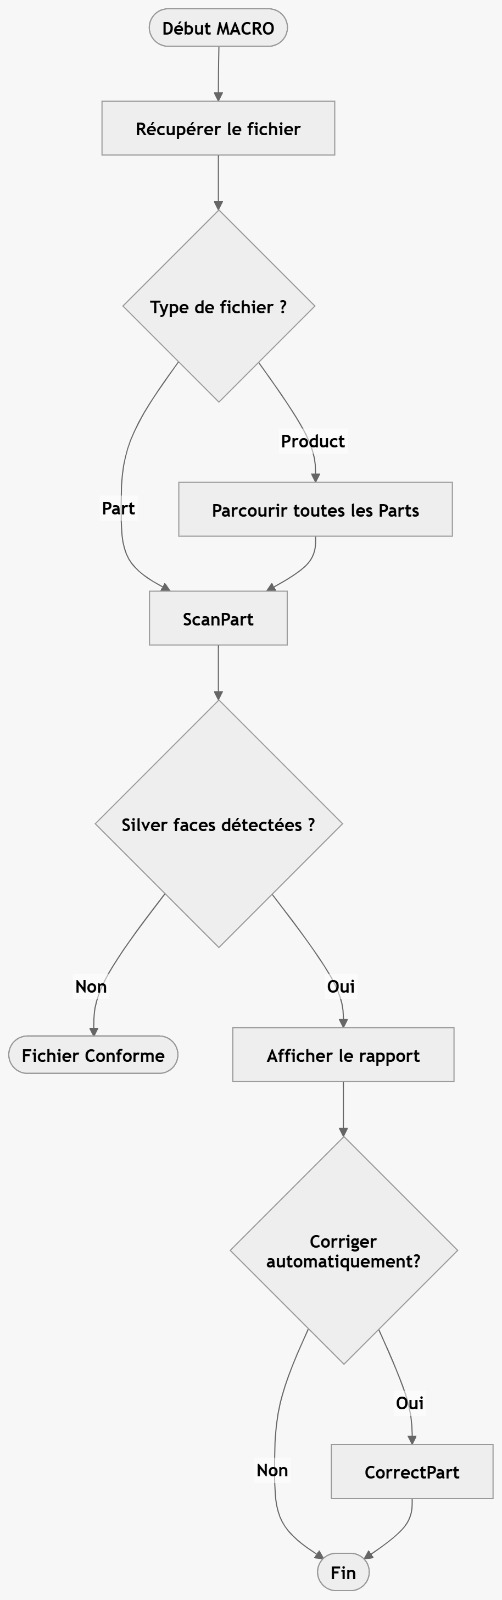
\includegraphics[height=0.85\textheight,keepaspectratio]{image/SILVER-FACE/CatMain_Silver_Face_TD.jpeg}
    \caption{Organigramme de la fonction \texttt{CATMain()} --- vue globale de la macro.}
    \label{fig:sf-flowchart-catmain}
\end{figure}

\subsubsection{Étape 2: \texttt{ScanPart()}}
\label{subsubsec:sf-scanpart}

Cette fonction inspecte l'ensemble des surfaces du Part et mesure leur aire.

La mesure utilise le \textbf{SPAWorkbench} de CATIA via l'objet \texttt{Measurable}. La propriété \texttt{.Area} est retournée en $\text{m}^2$ puis convertie en $\text{mm}^2$ (× 1\,000\,000).

Pour chaque silver face détectée, sont enregistrés : son nom, le Part et le dossier la contenant, son aire exacte en $\text{mm}^2$, et la stratégie de réparation associée :
\begin{itemize}
    \item[•] \textbf{Suppression}: si (l'aire $< 0{,}0001\ \text{mm}^2$).
    \item[•] \textbf{Healing}: si 
    ($0{,}0001 \leq \text{aire} < 0{,}01\ \text{mm}^2$).
\end{itemize}

\begin{figure}[htbp]
    \centering
    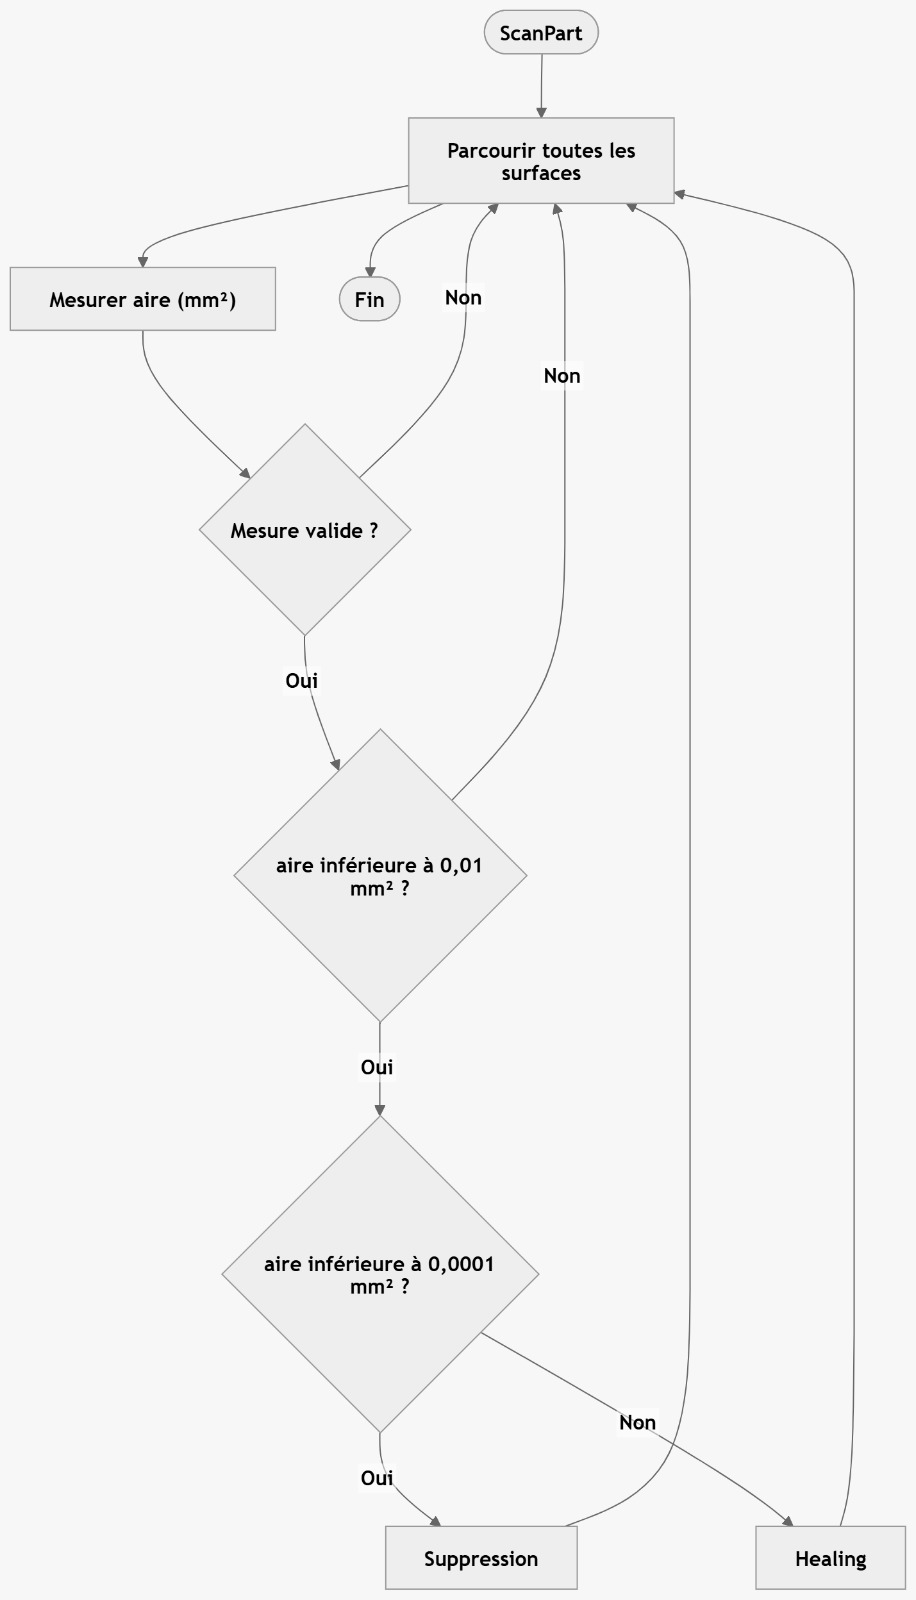
\includegraphics[height=0.85\textheight,keepaspectratio]{image/SILVER-FACE/ScanPart_Silver_Face_TD.jpeg}
    \caption{Organigramme de la fonction \texttt{ScanPart()} --- détection des silver faces.}
    \label{fig:sf-flowchart-scanpart}
\end{figure}

\subsubsection{Étape 3: \texttt{CorrigerPart()}}
\label{subsubsec:sf-corriger}

Cette fonction applique deux stratégies de correction automatique.

\paragraph{Suppression directe}
Appliquée lorsque l'aire est inférieure à $0{,}0001\ \text{mm}^2$. La surface est sélectionnée via \texttt{Selection.Add} puis supprimée par \texttt{Selection.Delete}, reproduisant l'action manuelle d'un utilisateur qui sélectionne et efface l'élément. La boucle se déroule \textbf{en sens inverse} pour éviter la désynchronisation des indices lors des suppressions successives.

\paragraph{Healing}
Le \textbf{Healing} est un outil de réparation CATIA qui:
\begin{enumerate}
    \item[•] prend un ensemble de surfaces ;
    \item[•] détecte les micro-écarts ou chevauchements entre elles ;
    \item[•] comble ou ferme ces écarts dans la tolérance \texttt{HEALING\_DIST} = $0{,}1\ \text{mm}$ ;
    \item[•] produit un groupe de surfaces « guéri » exempt de silver faces.
\end{enumerate}

\begin{figure}[htbp]
    \centering
    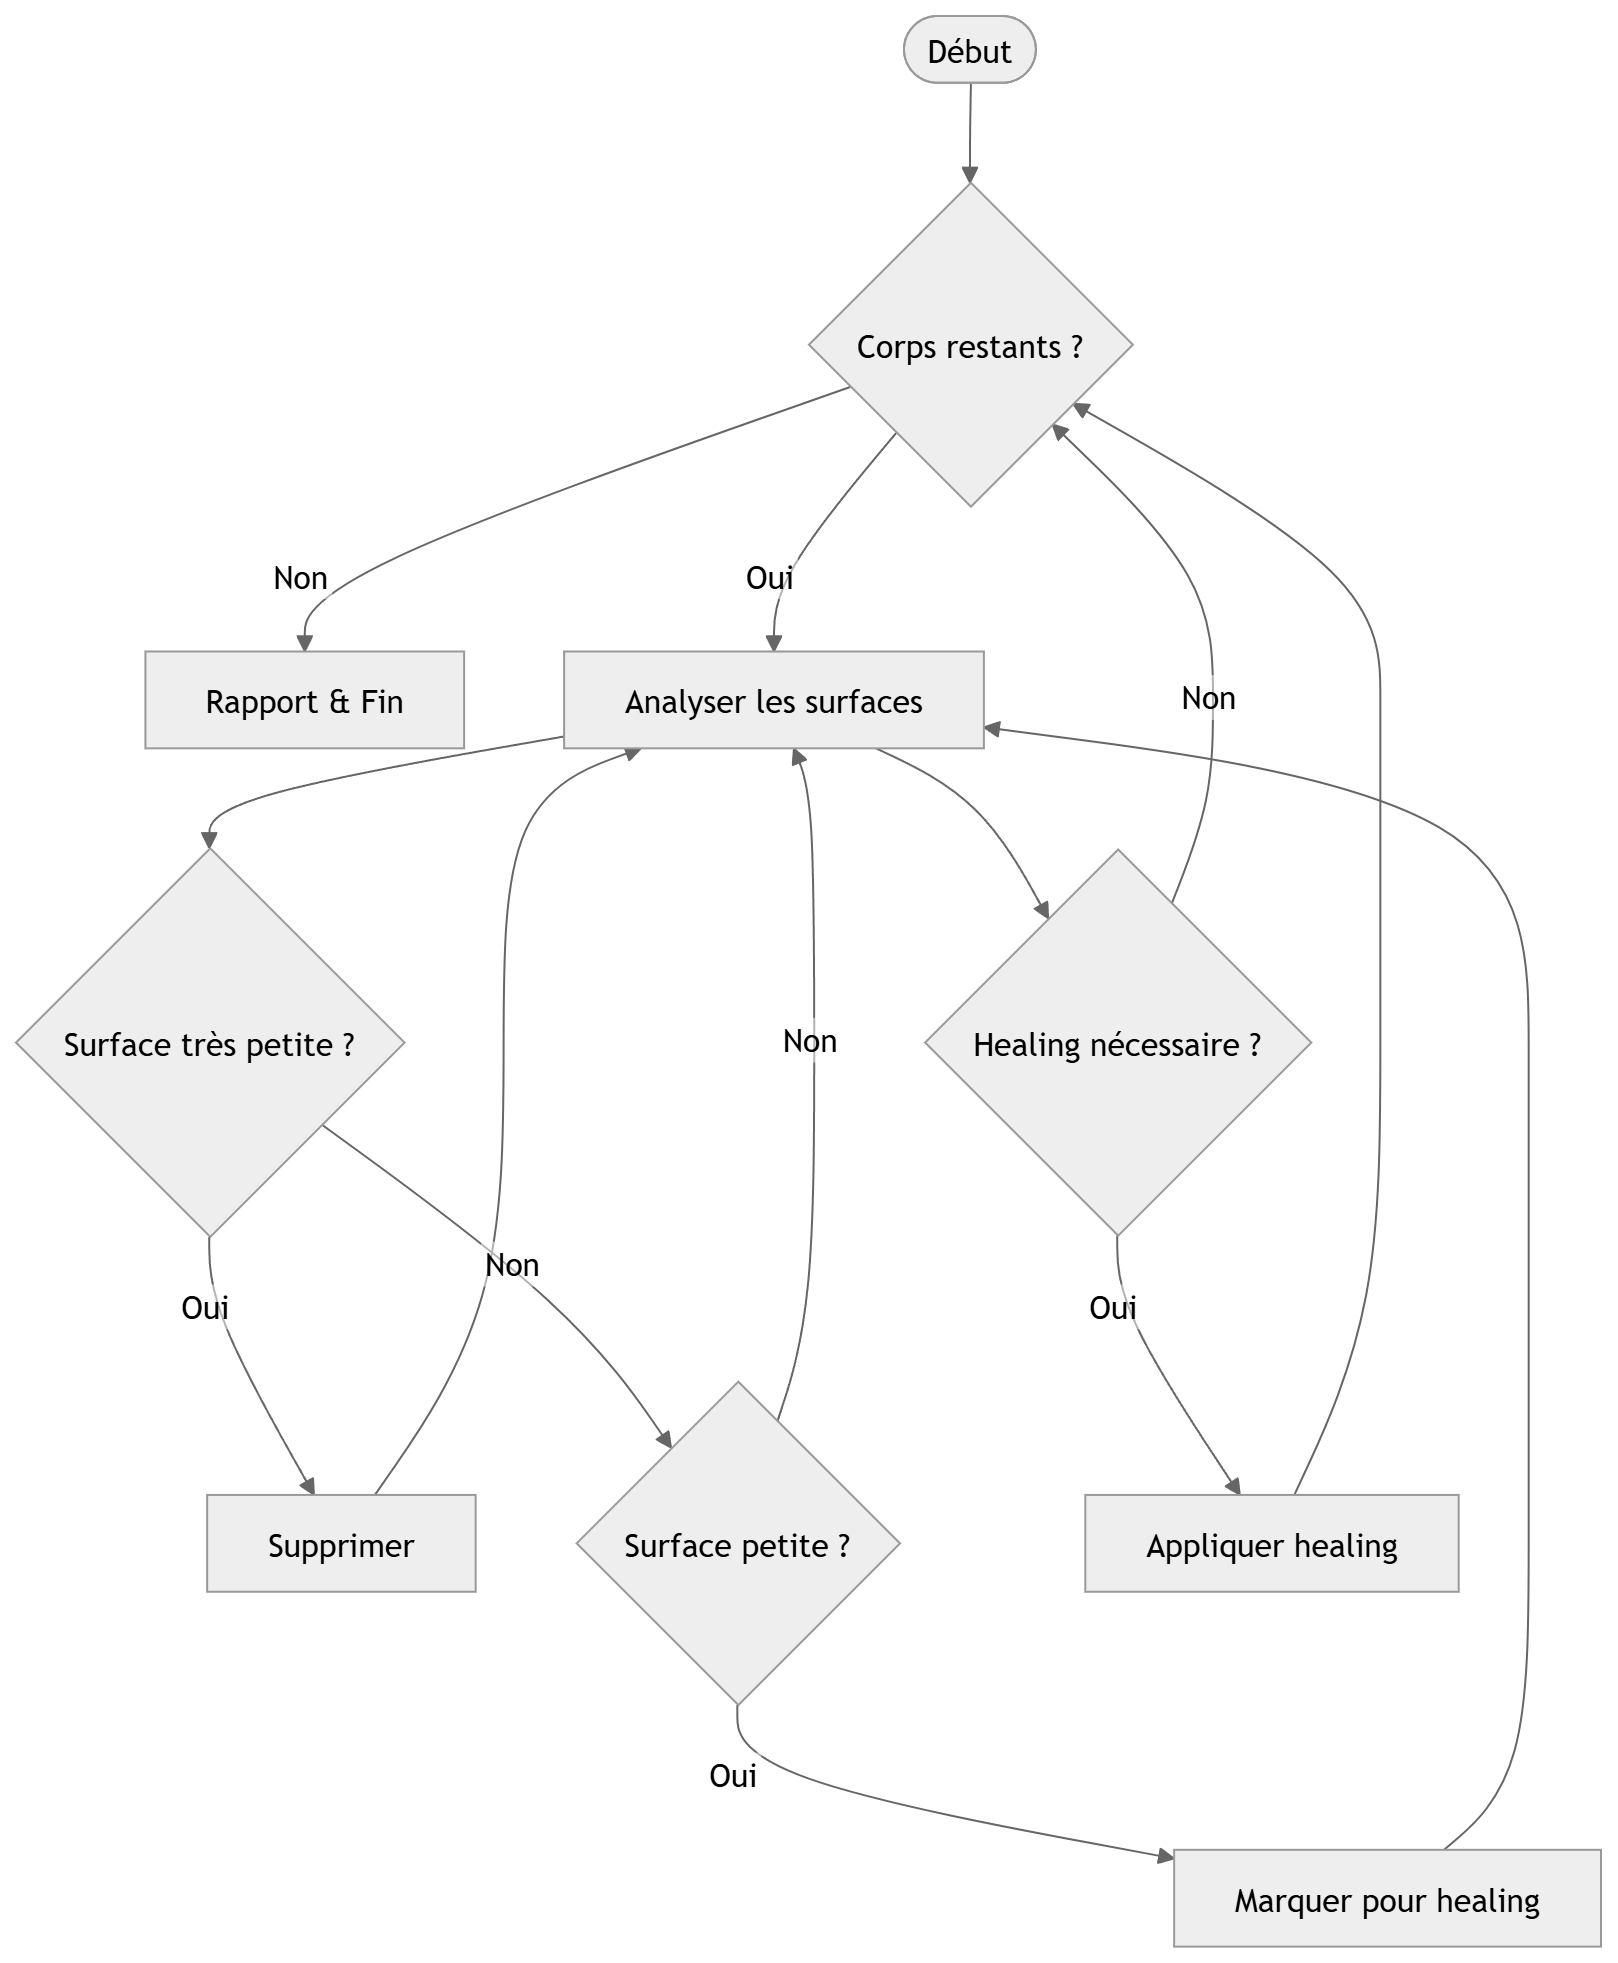
\includegraphics[height=0.85\textheight,keepaspectratio]{image/SILVER-FACE/Corriger_silver_face_TD.png}
    \caption{Organigramme de la fonction \texttt{CorrigerPart()} --- stratégies de correction.}
    \label{fig:sf-flowchart-corriger}
\end{figure}
\chapter{Innover}
\label{cp:innover}

La phase \textit{Innover} de la démarche DMAIC vise à concevoir des solutions nouvelles permettant de supprimer les causes racines des non-conformités identifiées lors des phases précédentes. Dans ce projet, l'innovation porte sur l'intégration d'un modèle d'apprentissage automatique pour détecter automatiquement les \textit{silver faces} $\bullet$ des surfaces dégénérées difficiles à identifier par une règle déterministe simple.

Ce chapitre présente l'approche complète : extraction des caractéristiques géométriques, construction du modèle de régression logistique, analyse des performances et recommandations pour la mise en production dans un pipeline CATIA~V5.

% ============================================================
\section{Détection des \textit{Silver Faces} par Régression Logistique}
\label{sec:innover-silver-faces}
% ============================================================

\subsection{Problématique}
\label{subsec:problematique}

La macro existante est entièrement \textbf{basée sur des règles} et utilise exactement \textbf{une seule caractéristique} pour prendre chaque décision~:

\begin{equation}
    \text{Aire}\;(\text{mm}^2) < 0{,}01 \;\Rightarrow\; \textit{silver face}
    \label{eq:decision-rule-old}
\end{equation}

Cette approche est fragile. Les deux constantes arbitraires $\bullet$ \texttt{SEUIL\_MM2~=~0.01} et \texttt{SEUIL\_DELETE~=~0.0001} $\bullet$ ont été fixées manuellement par un ingénieur. Elles ne peuvent pas s'adapter~:

\begin{itemize}
    \item \textbf{Aux domaines industriels différents} $\bullet$ les tolérances aérospatiales et automobiles diffèrent d'ordres de grandeur.
    \item \textbf{Aux styles de modélisation différents} $\bullet$ les pièces importées en IGES et les pièces modélisées nativement dans CATIA présentent des propriétés géométriques très différentes.
    \item \textbf{Au contexte} $\bullet$ une surface de $0{,}008~\text{mm}^2$ adjacente à une aube de turbine constitue un \textit{défaut critique}~; la même aire sur un panneau décoratif n'est que du \textit{bruit}.
\end{itemize}

L'apprentissage automatique remplace ces seuils figés par une \textbf{fonction de décision apprise} à partir de l'historique réel des corrections.

% ============================================================
\subsection{Caractéristiques géométriques utilisées}
\label{subsec:features}
% ============================================================

Quatre indicateurs géométriques sont extraits pour chaque surface afin de capturer sa forme de manière discriminante.

La \textbf{compacité} (ou quotient isopérimétrique) est la métrique la plus puissante. Elle mesure l'écart entre la forme d'une surface et un cercle parfait~:

\begin{equation}
    C = \frac{4\pi A}{P^2}, \qquad C \in (0,\,1]
    \label{eq:compacite}
\end{equation}

où $A$ désigne l'aire et $P$ le périmètre de la surface. Un cercle parfait donne $C = 1$~; une forme extrêmement allongée ou irrégulière tend vers $C \approx 0$. Le \textbf{rapport d'aspect} complète cette information en mesurant l'élongation directe de la boîte englobante~:

\begin{equation}
    AR = \frac{L_{\max}}{L_{\min}}
    \label{eq:aspect-ratio}
\end{equation}

où $L_{\max}$ et $L_{\min}$ désignent respectivement la plus grande et la plus petite dimension. Un carré donne $AR = 1$~; une \textit{silver face} typique présente $AR \gg 60$. Enfin, l'\textbf{aire} $A$ (en mm²) et le \textbf{périmètre} $P$ (en mm) fournissent une information brute sur la taille absolue de la surface.

La \autoref{fig:distribution} illustre la distribution de ces quatre caractéristiques sur l'ensemble des~1\,500 surfaces du jeu de données.

\begin{figure}[H]
    \centering
    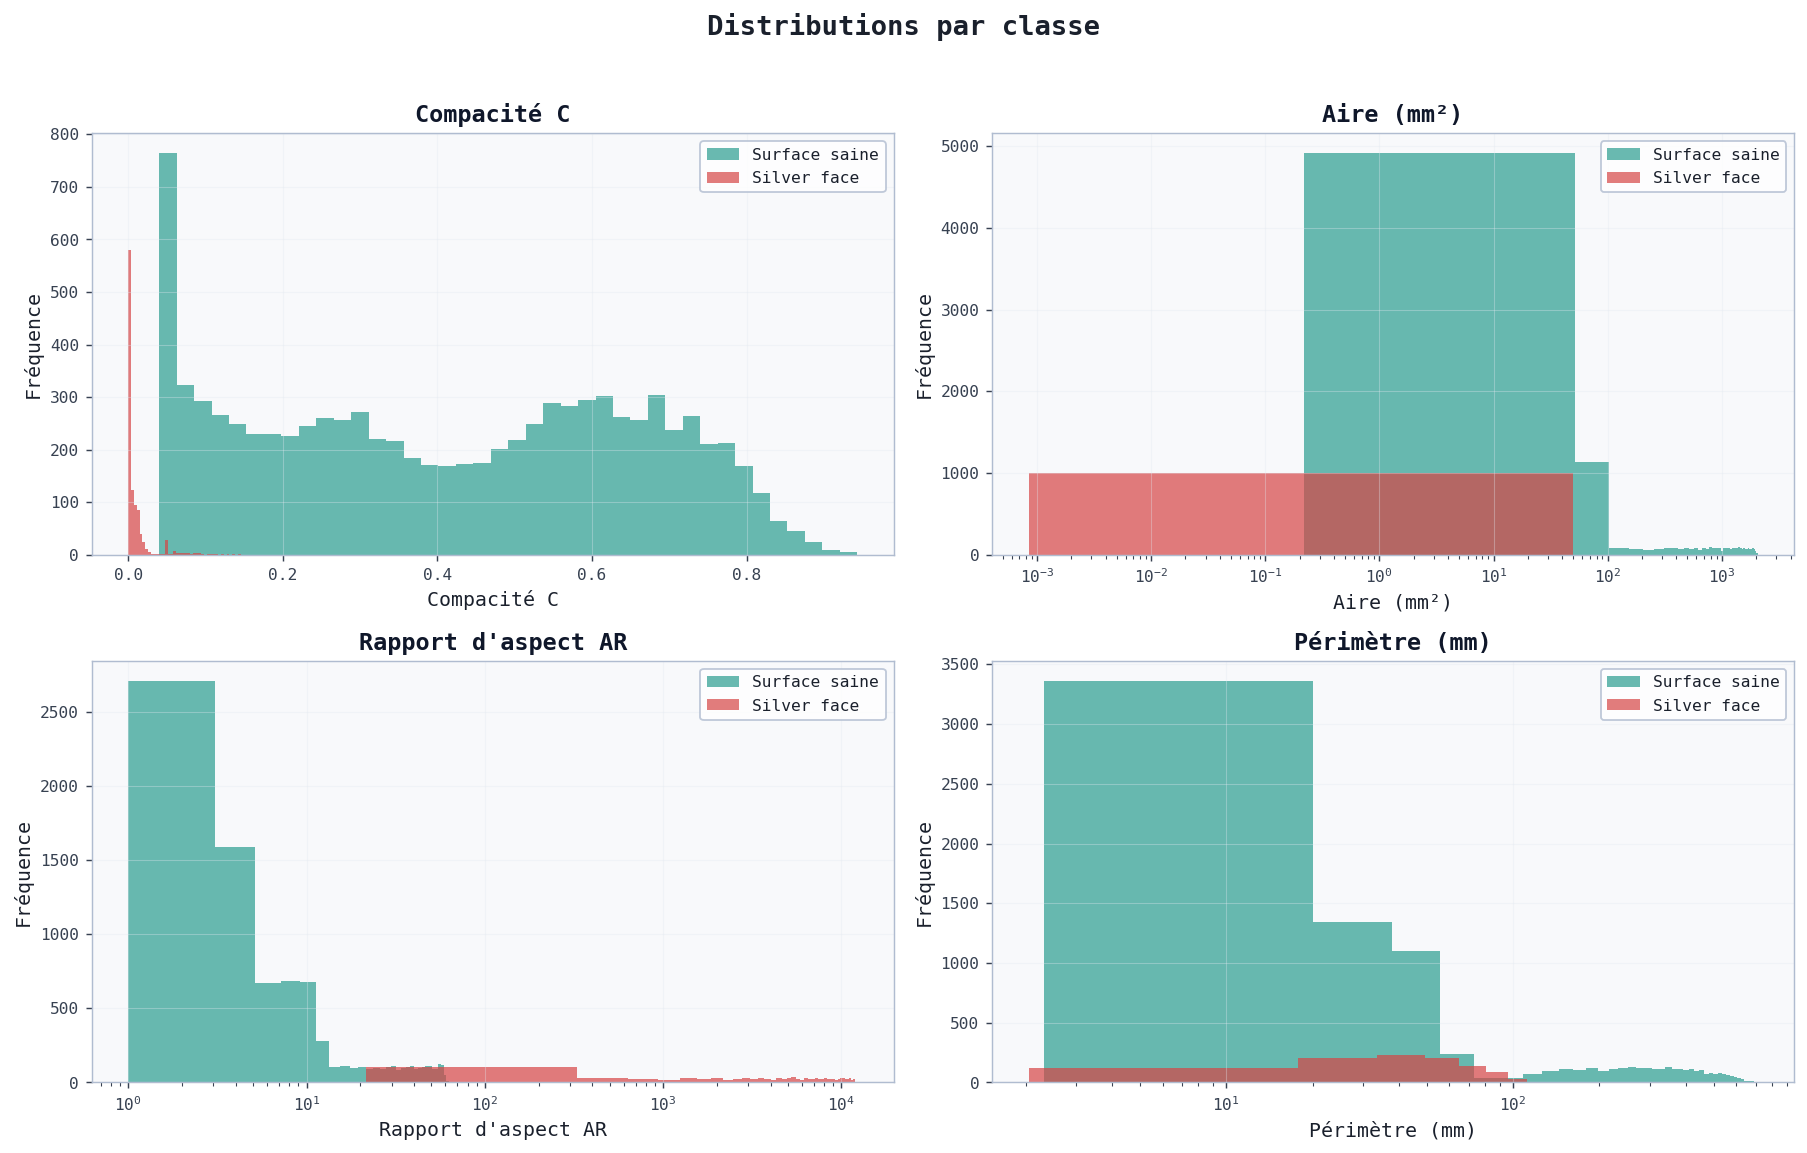
\includegraphics[width=\textwidth]{image/AI-SILVER-FACE/fig1_distribution.png}
    \caption{Distributions des quatre caractéristiques par classe (vert~: surface saine, rouge~: \textit{silver face}).}
    \label{fig:distribution}
\end{figure}

L'analyse de ces distributions révèle que la \textbf{compacité} et le \textbf{rapport d'aspect} sont les caractéristiques les plus discriminantes au premier degré~: les deux classes présentent des distributions quasi disjointes pour ces deux indicateurs. À l'inverse, l'aire et le périmètre offrent une séparation partielle mais insuffisante à eux seuls $\bullet$ ils jouent un rôle d'affinage dans les cas ambigus.

% ============================================================
\subsection{Espace des caractéristiques}
\label{subsec:feature-space}
% ============================================================

La \autoref{fig:feature-space} représente la distribution des 1\,500 surfaces dans l'espace des caractéristiques. Les surfaces saines apparaissent en vert, les \textit{silver faces} en rouge.

\begin{figure}[H]
    \centering
    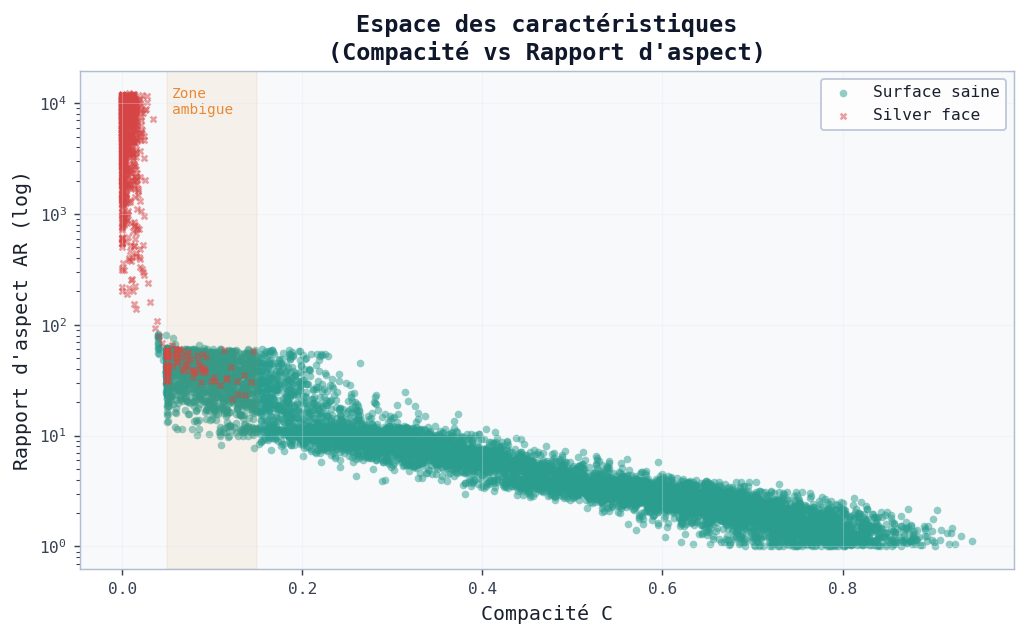
\includegraphics[width=0.9\textwidth]{image/AI-SILVER-FACE/fig2_feature_space.png}
    \caption{Compacité $C$ vs rapport d'aspect $AR$ : cluster \textit{silver face} (rouge) à faible $C$ et $AR$ élevé ; zone ambiguë en beige.}
    \label{fig:feature-space}
\end{figure}

Dans le plan Compacité $\times$ Rapport d'aspect, les deux classes se séparent nettement~: les \textit{silver faces} occupent la région de faible compacité ($C < 0{,}15$) et de rapport d'aspect élevé ($AR > 60$), tandis que les surfaces saines se concentrent dans la région de forte compacité ($C > 0{,}5$) et de faible rapport d'aspect ($AR < 20$). La zone d'ambiguïté, encadrée en beige, correspond à $C \in [0{,}05,\, 0{,}15]$ et $AR \in [30,\, 60]$~: des surfaces saines très allongées peuvent y coexister avec des \textit{silver faces} modérées.

Cette visualisation confirme le rôle central de la compacité $C$ et du rapport d'aspect $AR$ comme caractéristiques principales du modèle~: leur pouvoir discriminant est maximal, et leur combinaison permet de délimiter une frontière de décision claire et robuste. Le modèle de régression logistique exploite précisément cette structure géométrique pour séparer les deux classes avec un minimum de mauvaises classifications.

% ============================================================
\section{Modèle : Régression Logistique}
\label{sec:modele-rl}
% ============================================================

\subsection{Normalisation des données}
\label{subsec:normalisation}

Avant l'entraînement, chaque caractéristique est normalisée par le \textbf{z-score} calculé sur le jeu d'entraînement uniquement, afin d'éviter toute fuite de données vers le jeu de test :

\begin{equation}
    z_i = \frac{x_i - \mu_i}{\sigma_i}
    \label{eq:zscore}
\end{equation}

où les symboles sont définis dans le \autoref{tab:zscore-symbols}.

\begin{table}[H]
    \centering
    \caption{Symboles de la normalisation par z-score}
    \label{tab:zscore-symbols}
    \begin{tabularx}{\textwidth}{|>{\bfseries\centering\arraybackslash}p{2cm}|X|}
        \hline
        \rowcolor{headerblue}
        \textcolor{white}{\textbf{Symbole}} & \centering\textcolor{white}{\textbf{Définition}} \tabularnewline
        \hline
        \rowcolor{rowlight}
        $x_i$ & Valeur brute de la caractéristique $i$ \\
        \hline
        \rowcolor{rowwhite}
        $\mu_i$ & Moyenne calculée sur le jeu d'entraînement \\
        \hline
        \rowcolor{rowlight}
        $\sigma_i$ & Écart-type calculé sur le jeu d'entraînement \\
        \hline
    \end{tabularx}
\end{table}

Cette étape est indispensable : les caractéristiques ont des ordres de grandeur très différents (l'aire peut valoir 2\,000~mm² tandis que la compacité vaut 0.001), ce qui déséquilibrerait sinon le processus d'optimisation.

\subsection{Fonction de décision}
\label{subsec:decision-function}

La régression logistique associe à chaque surface un score linéaire $z$, puis le transforme en probabilité via la \textbf{fonction sigmoïde} :

\begin{equation}
    P(\text{\textit{silver face}} \mid \mathbf{x}) = \sigma(z) = \frac{1}{1 + e^{-z}}, \qquad z = \mathbf{w}^\top \tilde{\mathbf{x}} + b
    \label{eq:sigmoid}
\end{equation}

où $\mathbf{w}$ est le vecteur des poids appris, $\tilde{\mathbf{x}}$ le vecteur des caractéristiques normalisées, et $b$ le biais.

La décision finale dépend d'un \textbf{seuil de classification} $\tau$ :

\begin{equation}
    \hat{y} = \begin{cases}
        1 \text{ (\textit{silver face})} & \text{si } P \geq \tau \\
        0 \text{ (surface saine)}        & \text{sinon}
    \end{cases}
    \label{eq:decision}
\end{equation}

% ============================================================
\section{Analyse des résultats}
\label{sec:resultats}
% ============================================================

\subsection{Courbe sigmoïde, distributions et courbes de performance}
\label{subsec:analyse-complete}

\begin{figure}[H]
    \centering
    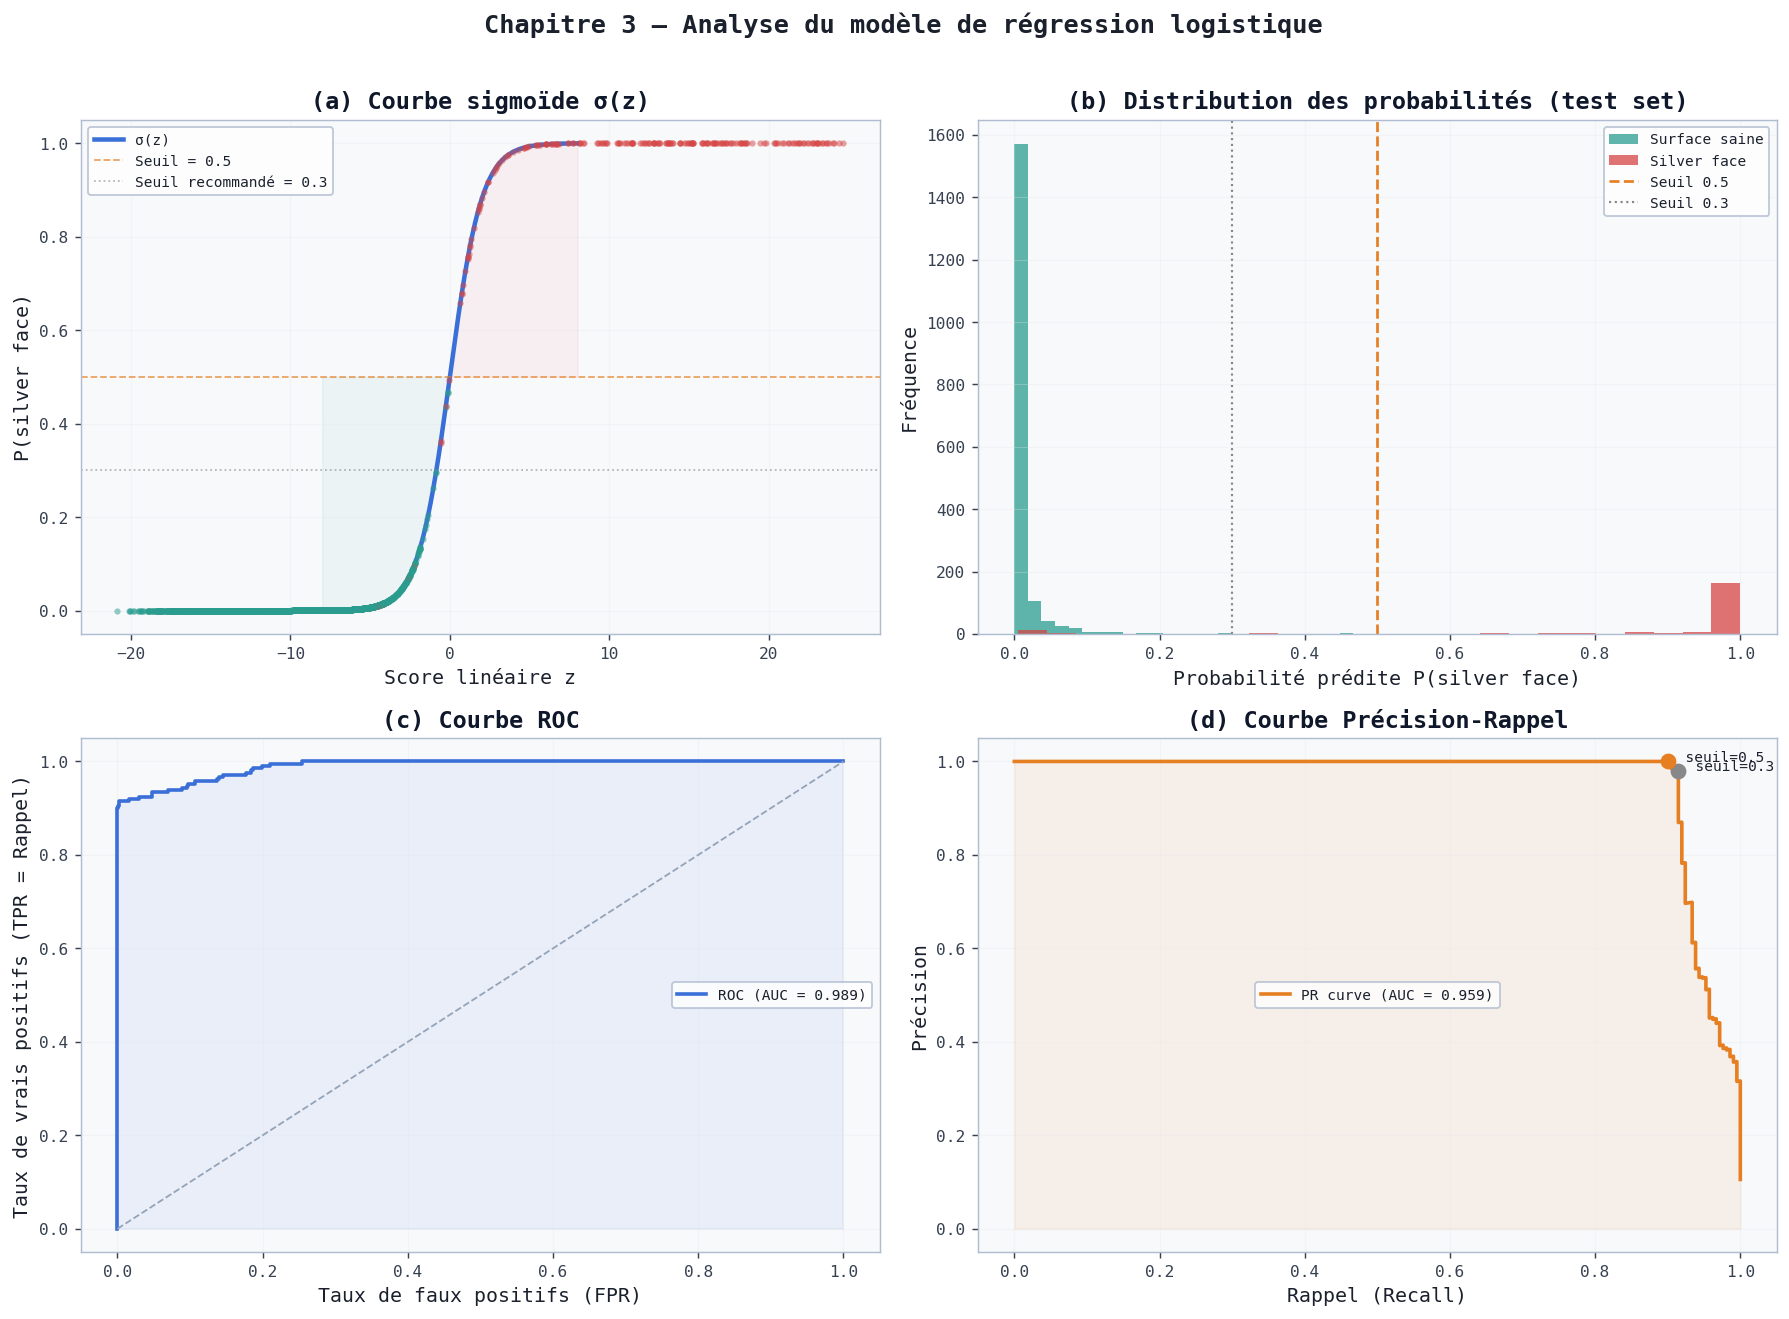
\includegraphics[width=\textwidth]{image/AI-SILVER-FACE/fig3_analysis.png}
    \caption{Analyse du modèle sur le jeu de test : (a)~sigmoïde $\sigma(z)$, (b)~distribution des probabilités prédites, (c)~courbe ROC (AUC~=~0,989), (d)~courbe Précision-Rappel (AUC~=~0,959).}
    \label{fig:analysis}
\end{figure}

Le panneau~(a) montre que chaque surface projetée sur la courbe sigmoïde selon son score linéaire $z$ se sépare nettement en deux nuages~; les rares points autour de $z \approx 0$ correspondent aux cas ambigus de la zone de chevauchement. Le panneau~(b) visualise le \textbf{recouvrement} entre les deux distributions~: plus les deux histogrammes sont séparés et étroits, plus le modèle est confiant.

La courbe ROC (panneau~c) représente le compromis entre le \textbf{taux de vrais positifs} (rappel, TPR) et le \textbf{taux de faux positifs} (FPR) pour tous les seuils $\tau$ possibles~:

\begin{equation}
    \text{TPR} = \frac{VP}{VP + FN}, \qquad \text{FPR} = \frac{FP}{FP + VN}
    \label{eq:tpr-fpr}
\end{equation}

La courbe PR (panneau~d) est particulièrement adaptée aux \textbf{jeux de données déséquilibrés} (ici 73~\% saines / 27~\% \textit{silver faces}). Elle représente le compromis entre~:

\begin{equation}
    \text{Précision} = \frac{VP}{VP + FP}, \qquad \text{Rappel} = \frac{VP}{VP + FN}
    \label{eq:precision-rappel}
\end{equation}

Dans un contexte de contrôle qualité, le \textbf{rappel} est prioritaire $\bullet$ manquer une \textit{silver face} (faux négatif) est plus coûteux qu'une fausse alarme. Un seuil abaissé à $\tau = 0{,}3$ augmente le rappel au prix d'une légère diminution de la précision.

\subsection{Frontière de décision}
\label{subsec:decision-boundary}

\begin{figure}[H]
    \centering
    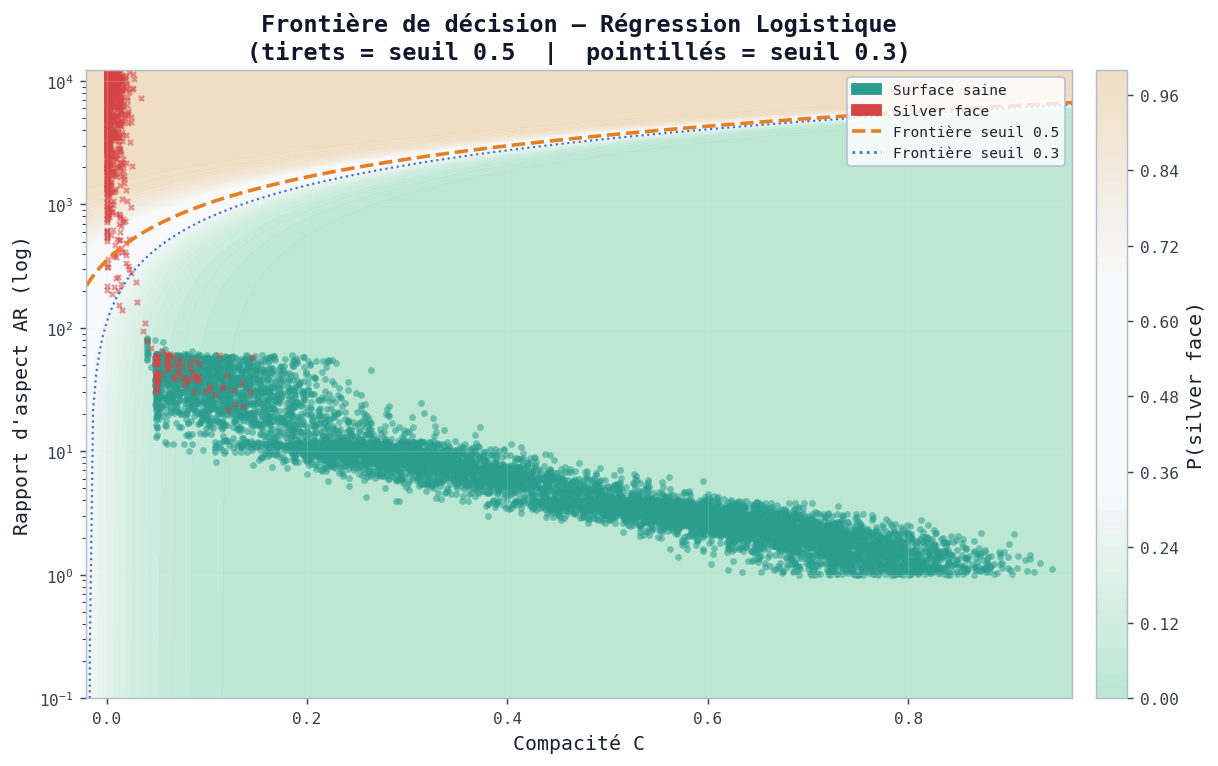
\includegraphics[width=0.9\textwidth]{image/AI-SILVER-FACE/fig4_decision_boundary.png}
    \caption{Frontière de décision dans le plan $C \times AR$ (tirets~: $\tau = 0{,}5$~; pointillés~: $\tau = 0{,}3$).}
    \label{fig:decision-boundary}
\end{figure}

Le seuil $\tau = 0.3$ est décalé vers la zone saine, ce qui permet de capturer davantage de \textit{silver faces} au prix d'un léger empiétement sur les surfaces saines ambiguës.

% ============================================================
\section{Métriques de classification}
\label{sec:metriques}
% ============================================================

Les matrices de confusion quantifient les performances du modèle pour les deux seuils de classification étudiés.

\subsection{Seuil standard \texorpdfstring{$\tau = 0.5$}{tau = 0.5}}
\label{subsec:confusion-05}

\begin{figure}[H]
    \centering
    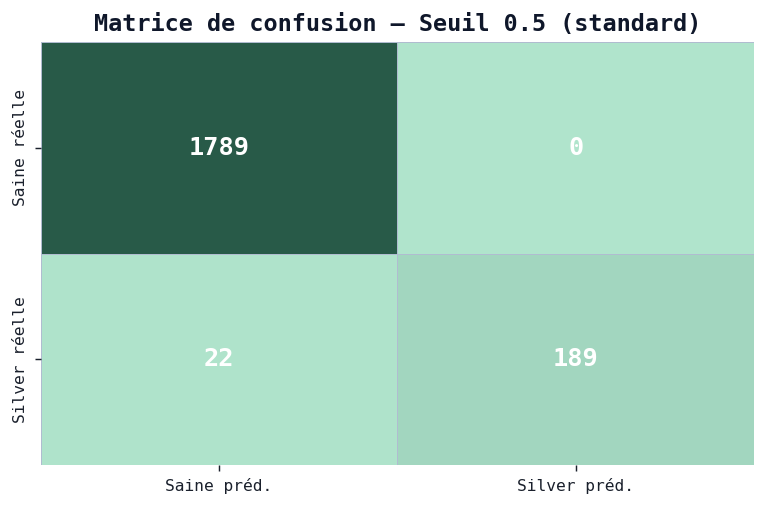
\includegraphics[width=0.65\textwidth]{image/AI-SILVER-FACE/fig5a_confusion_05.png}
    \caption{Matrice de confusion $\bullet$ seuil standard $\tau = 0{,}5$.}
    \label{fig:confusion-05}
\end{figure}

\subsection{Seuil recommandé \texorpdfstring{$\tau = 0.3$}{tau = 0.3}}
\label{subsec:confusion-03}

\begin{figure}[H]
    \centering
    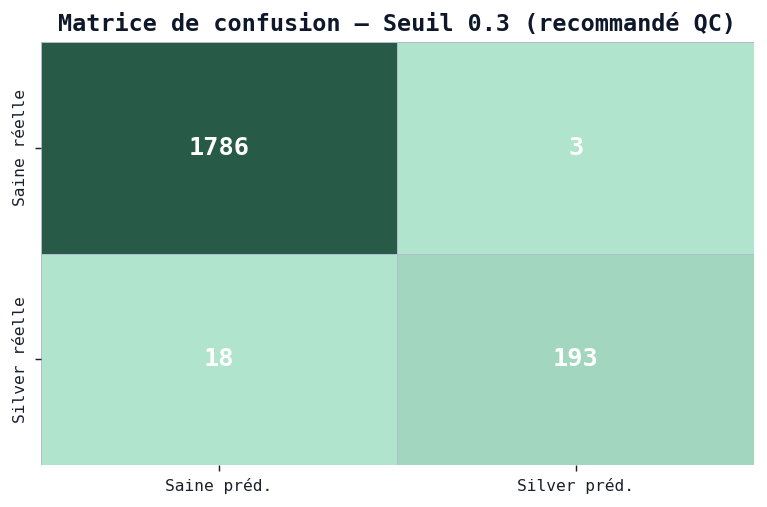
\includegraphics[width=0.65\textwidth]{image/AI-SILVER-FACE/fig5b_confusion_03.png}
    \caption{Matrice de confusion $\bullet$ seuil recommandé $\tau = 0{,}3$.}
    \label{fig:confusion-03}
\end{figure}

Les quatre cases de la matrice de confusion sont définies dans le \autoref{tab:confusion-matrix-def}.

\begin{table}[H]
    \centering
    \caption{Définition des cases de la matrice de confusion}
    \label{tab:confusion-matrix-def}
    \begin{tabularx}{\textwidth}{|X|>{\centering\arraybackslash}p{4cm}|>{\centering\arraybackslash}p{4.5cm}|}
        \hline
        \rowcolor{headerblue}
        \textcolor{white}{\textbf{}} &
        \textcolor{white}{\textbf{Prédit saine}} &
        \textcolor{white}{\textbf{Prédit \textit{silver face}}} \tabularnewline
        \hline
        \rowcolor{rowlight}
        \textbf{Réelle saine} & Vrais négatifs (VN) & Faux positifs (FP) \\
        \hline
        \rowcolor{rowwhite}
        \textbf{Réelle \textit{silver face}} & Faux négatifs (FN) & Vrais positifs (VP) \\
        \hline
    \end{tabularx}
\end{table}

Avec le seuil standard $\tau = 0.5$, le modèle ne classe \textit{silver face} que les cas très probables, réduisant les faux positifs mais augmentant le risque de faux négatifs. Avec $\tau = 0.3$, le modèle est plus sensible et détecte davantage de \textit{silver faces} réelles au prix de quelques fausses alarmes supplémentaires. Dans un pipeline de contrôle qualité automatisé, ce compromis est préférable.

% ============================================================
\section{Interprétabilité $\bullet$ Poids du modèle}
\label{sec:interpretabilite}
% ============================================================

\begin{figure}[H]
    \centering
    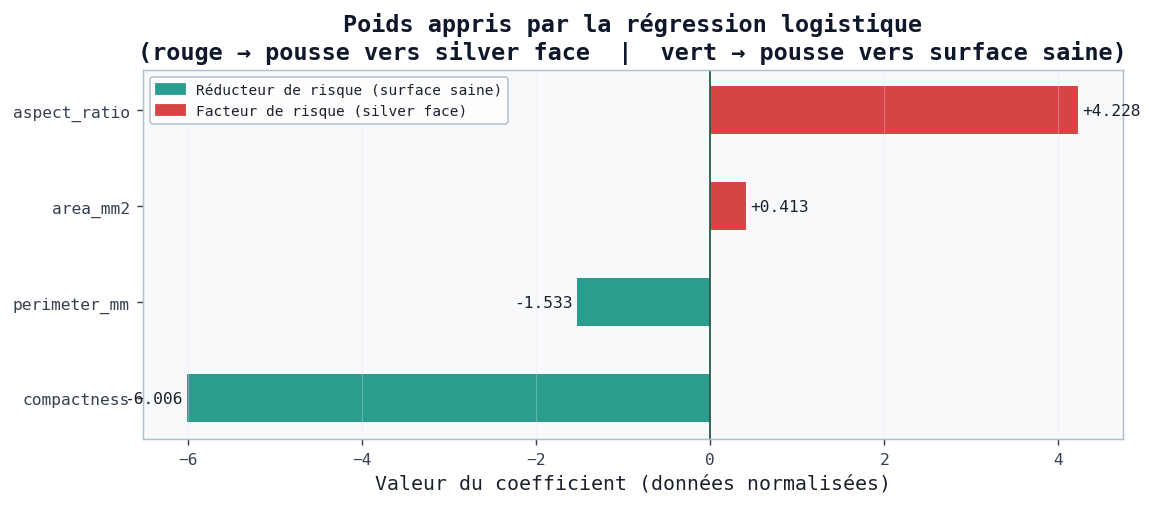
\includegraphics[width=0.85\textwidth]{image/AI-SILVER-FACE/fig6_weights.png}
    \caption{Coefficients appris par la régression logistique (rouge~: facteur de risque, vert~: réducteur de risque).}
    \label{fig:weights}
\end{figure}

Les poids $w_i$ indiquent la contribution de chaque caractéristique normalisée à la décision finale :

\begin{itemize}
    \item Le \textbf{rapport d'aspect} ($AR$, coefficient $+4.228$) est le facteur le plus influent en faveur d'une détection \textit{silver face} : plus $AR$ est élevé, plus la surface est suspecte.
    \item La \textbf{compacité} ($C$, coefficient $-6.006$) est le facteur protecteur dominant : une compacité élevée est une forte indication de surface saine.
    \item L'\textbf{aire} et le \textbf{périmètre} jouent un rôle secondaire, affinant la décision dans les cas ambigus.
\end{itemize}

% ============================================================
\section{Conclusion et recommandations}
\label{sec:innover-conclusion}
% ============================================================

Le modèle de régression logistique entraîné sur 1\,500 surfaces synthétiques démontre une capacité de discrimination robuste entre surfaces saines et \textit{silver faces}, avec une AUC-ROC de 0.989 et une AUC-PR de 0.959.

\textbf{Recommandations pour la mise en production :}

\begin{enumerate}
    \item \textbf{Seuil de classification} : utiliser $\tau = 0.3$ plutôt que le seuil standard 0.5, afin de maximiser la détection des \textit{silver faces} dans un contexte de contrôle qualité.
    \item \textbf{Indicateurs à surveiller} : la compacité $C$ et le rapport d'aspect $AR$ sont les deux signaux les plus discriminants. Une surface avec $C < 0.05$ et $AR > 100$ doit être systématiquement signalée.
    \item \textbf{Intégration CATIA} : le modèle peut être appelé depuis un script VBScript (\texttt{silver\_faces.vbs}) en extrayant les quatre caractéristiques géométriques via les APIs de mensuration CATIA~V5.
\end{enumerate}

\chapter{Contrôler}
\label{cp:controler}

\textit{À compléter.}

% \chapter[Exemples de Mise en Forme: Guide des Éléments LaTeX]{Exemples de Mise en Forme Guide des Éléments LaTeX}
\label{cp:examples}

Ce chapitre présente des exemples de tous les éléments de mise en forme disponibles dans ce modèle LaTeX. Vous pouvez utiliser ce chapitre comme référence pour voir comment chaque élément apparaît dans le document final.

\section{Titres et Sections}
Les sections permettent d'organiser votre document de manière hiérarchique.

\subsection{Sous-section}
Ceci est un exemple de sous-section. Les sous-sections sont utilisées pour diviser une section en parties plus petites.

\subsubsection{Sous-sous-section}
Ceci est un exemple de sous-sous-section, le niveau le plus bas de la hiérarchie des titres.

\section{Texte et Mise en Forme}

\subsection{Styles de Texte}
Voici différents styles de texte disponibles:

\begin{itemize}
    \item \textbf{Texte en gras} -- utiliser \verb|\textbf{}|
    \item \textit{Texte en italique} -- utiliser \verb|\textit{}|
    \item \underline{Texte souligné} -- utiliser \verb|\underline{}|
    \item \texttt{Texte monospace} -- utiliser \verb|\texttt{}|
    \item \textsc{Petites Capitales} -- utiliser \verb|\textsc{}|
\end{itemize}

\subsection{Citations et Blocs}

\begin{block}[note]
Ceci est un bloc de note. Il est utilisé pour mettre en évidence des informations importantes que le lecteur devrait remarquer.
\end{block}

\begin{block}[tip]
Ceci est un bloc de conseil. Il fournit des astuces utiles ou des bonnes pratiques.
\end{block}

\section{Listes}

\subsection{Liste à Puces}
\begin{itemize}
    \item Premier élément de la liste
    \item Deuxième élément de la liste
    \item Troisième élément de la liste
    \begin{itemize}
        \item Sous-élément A
        \item Sous-élément B
    \end{itemize}
\end{itemize}

\subsection{Liste Numérotée}
\begin{enumerate}
    \item Premier élément numéroté
    \item Deuxième élément numéroté
    \item Troisième élément numéroté
    \begin{enumerate}
        \item Sous-élément numéroté
        \item Autre sous-élément
    \end{enumerate}
\end{enumerate}

\subsection{Liste de Description}
\begin{description}
    \item[AI] Intelligence Artificielle -- technologie permettant aux machines d'apprendre.
    \item[Q-Checker] Outil de vérification de qualité géométrique.
    \item[CAO] Conception Assistée par Ordinateur.
\end{description}

\section{Tableaux}

\subsection{Tableau Simple}
\begin{table}[!htpb]
    \caption{Exemple de tableau simple avec l'environnement tabular.}
    \label{tab:exemple-simple}
    \centering
    \begin{tabular}{llc}
        \toprule
        \textbf{Paramètre} & \textbf{Description} & \textbf{Valeur} \\ 
        \midrule
        Épaisseur          & Épaisseur de la pièce    & 2.5 mm  \\
        Rayon              & Rayon de courbure        & 10 mm   \\
        Tolérance          & Tolérance géométrique    & 0.1 mm  \\
        \bottomrule
    \end{tabular}
\end{table}

\subsection{Tableau avec Colonnes Étendues}
\begin{table}[!htpb]
    \caption{Exemple de tableau avec l'environnement tabularx.}
    \label{tab:exemple-tabularx}
    \begin{tabularx}{\textwidth}{lX}
        \toprule
        \textbf{Composant} & \textbf{Description} \\ 
        \midrule
        Module AI & Ce module utilise des algorithmes d'apprentissage automatique pour analyser et optimiser la géométrie des pièces. \\
        Q-Checker & Outil de vérification qui valide la conformité géométrique des pièces selon les normes industrielles. \\
        Interface & Interface utilisateur permettant la visualisation et l'interaction avec les résultats d'optimisation. \\
        \bottomrule
    \end{tabularx}
\end{table}

\subsection{Tableau Complexe}
\begin{table}[!htpb]
    \caption{Exemple de tableau complexe avec multi-lignes.}
    \label{tab:exemple-complexe}
    \centering
    \begin{tabular}{lcc}
        \toprule
        \multirow{2}{*}{\textbf{Module}} & \multicolumn{2}{c}{\textbf{Caractéristiques}} \\
        \cmidrule(lr){2-3}
        & \textbf{Fonctionnalité} & \textbf{Actif} \\
        \midrule
        \multirow{3}{*}{Analyse} & Détection des défauts & $\checkmark$ \\
        & Mesure automatique & $\checkmark$ \\
        & Rapport PDF & $\checkmark$ \\
        \midrule
        \multirow{3}{*}{Optimisation} & Suggestion de corrections & $\checkmark$ \\
        & Apprentissage adaptatif & $\checkmark$ \\
        & Export CAO & - \\
        \bottomrule
    \end{tabular}
\end{table}

\section{Figures}

\begin{figure}[!htpb]
    \centering
    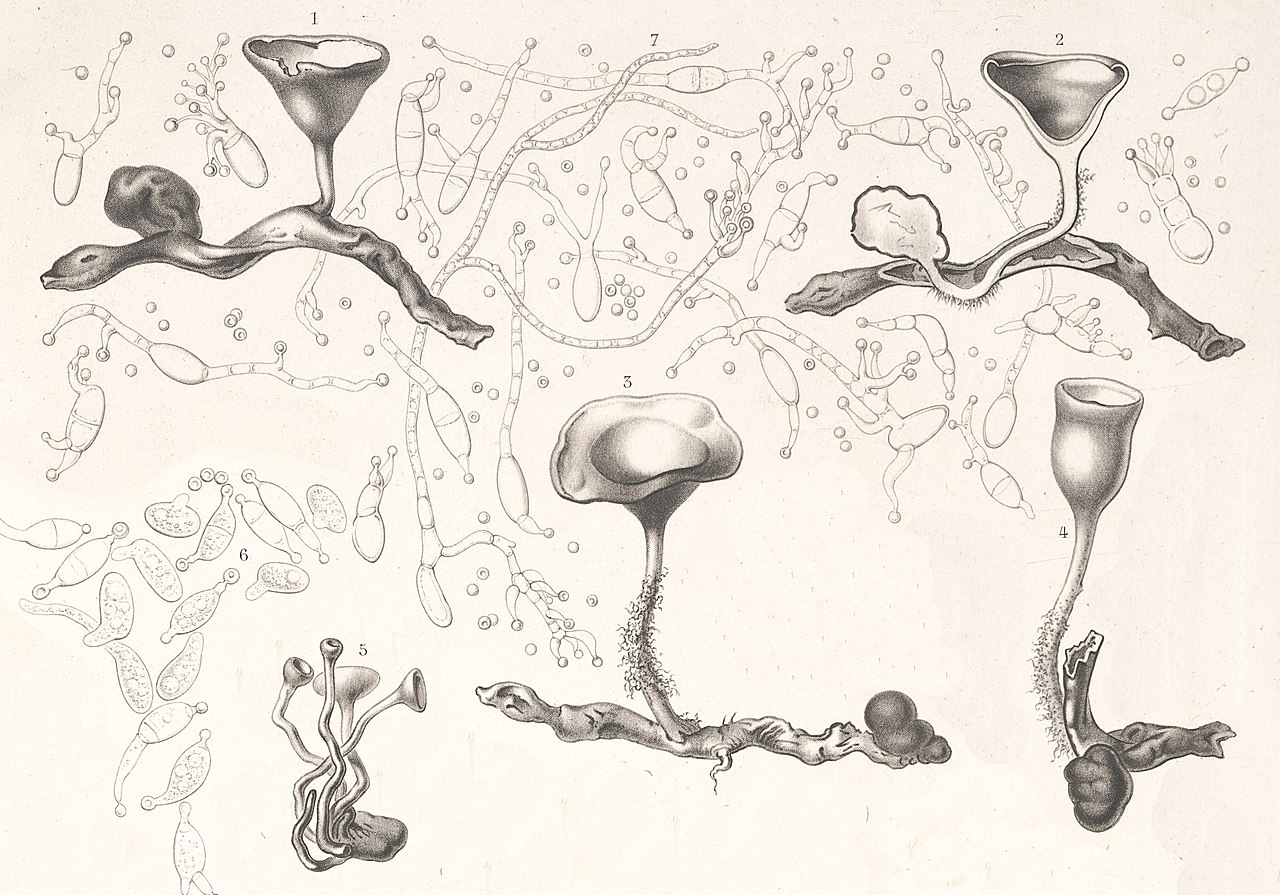
\includegraphics[width=0.7\linewidth]{Figures/PezizaTuberosa.jpg}
    \caption[Exemple de figure simple]{Exemple de figure simple. Remplacez cette image par vos propres figures pour illustrer votre travail.}
    \label{fig:exemple-figure}
\end{figure}

\section{Code Source}

\subsection{Code Inline}
Utilisez \verb|\verb| pour du code en ligne, par exemple: \verb|print("Hello World")|.

\subsection{Bloc de Code}
\begin{listing}[!htpb]
\caption{Exemple de code Python pour l'optimisation.}
\label{listing:python-exemple}
\begin{minted}{python}
import numpy as np

def optimize_geometry(parameters):
    """
    Fonction d'optimisation de géométrie.
    
    Args:
        parameters: Dictionnaire des paramètres géométriques
    
    Returns:
        Paramètres optimisés
    """
    # Algorithme d'optimisation
    optimized = {}
    for key, value in parameters.items():
        optimized[key] = value * 0.95  # Réduction de 5%
    
    return optimized

# Exemple d'utilisation
params = {"thickness": 2.5, "radius": 10.0}
result = optimize_geometry(params)
print(f"Résultat: {result}")
\end{minted}
\end{listing}

\subsection{Code depuis Fichier Externe}
\begin{listing}[!htpb]
\caption{Exemple de code Haskell importé depuis un fichier externe.}
\label{listing:haskell-exemple}
\inputminted{haskell}{Code/Factorial.hs}
\end{listing}

\subsection{Bloc Verbatim}
Pour afficher du texte brut sans mise en forme:

\begin{verbatim}
Ceci est un bloc verbatim.
Le texte est affiché tel quel,
sans aucune interprétation LaTeX.
\end{verbatim}

\section{Équations Mathématiques}

\subsection{Équation Inline}
La formule de la distance euclidienne est \(d = \sqrt{(x_2-x_1)^2 + (y_2-y_1)^2}\).

\subsection{Équation Numérotée}
\begin{equation}
\label{eq:optimization}
\min_{x} f(x) = \sum_{i=1}^{n} w_i \cdot (x_i - x_i^*)^2
\end{equation}

L'équation \ref{eq:optimization} représente une fonction objectif typique pour l'optimisation géométrique.

\subsection{Équation Sans Numéro}
\[
\mathcal{L}(\theta) = -\frac{1}{N} \sum_{i=1}^{N} \log P(y_i | x_i; \theta)
\]

\section{Références et Citations}

\subsection{Références Croisées}
Vous pouvez référencer des éléments du document:
\begin{itemize}
    \item Référence à un chapitre: \autoref{cp:examples}
    \item Référence à une section: \autoref{tab:exemple-simple}
    \item Référence à une figure: \autoref{fig:exemple-figure}
    \item Référence à une équation: Équation \ref{eq:optimization}
    \item Référence à un listing: \autoref{listing:python-exemple}
\end{itemize}

\subsection{Citations Bibliographiques}
Exemple de citation dans le texte: selon \citet{Elgamal1985}, les systèmes cryptographiques... 

Exemple de citation entre parenthèses: les méthodes de chiffrement modernes \citep{Elgamal1985}.

\section{Notes de Bas de Page}
Les notes de bas de page permettent d'ajouter des informations complémentaires\footnote{Ceci est un exemple de note de bas de page. Elle apparaît en bas de la page.}.

\section{Blocs Spéciaux}

\begin{block}[note]
\textbf{Note importante:} Ce modèle est conçu pour être flexible et s'adapter à différents types de documents académiques.
\end{block}

\begin{block}[tip]
\textbf{Conseil:} N'hésitez pas à consulter la documentation LaTeX pour découvrir d'autres fonctionnalités avancées.
\end{block}


% %%% Bibliography %%%
% \renewcommand{\refname}{Bibliographie}
% % \printbibliography[title={\refname},heading=bibintoc]

% %%% Appendices: Work that *YOU* Developed %%%
% \appendix
% \ifthenelse{\equal{\LanguageOption}{portuguese}}{
    \addtocontents{toc}{\protect\contentsline{chapter}{Apêndices}{}{}}
}{\ifthenelse{\equal{\LanguageOption}{spanish}}{
    \addtocontents{toc}{\protect\contentsline{chapter}{Apéndices}{}{}}
}{\ifthenelse{\equal{\LanguageOption}{french}}{
    \addtocontents{toc}{\protect\contentsline{chapter}{Annexes}{}{}}
}{
    \addtocontents{toc}{\protect\contentsline{chapter}{Appendices}{}{}}
}}}

\ifthenelse{\equal{\MediaOption}{paper}}{\blankpage}{\clearpage}
\begin{center}
    \crimsonfont
    \thispagestyle{empty}
        
    \vspace*{\fill}
    \ifthenelse{\equal{\LanguageOption}{portuguese}}{%
        {\LARGE\fontsize{26}{26}\selectfont\textcolor{ensablue}{Apêndices}\par}
    }{\ifthenelse{\equal{\LanguageOption}{spanish}}{%
        {\LARGE\fontsize{26}{26}\selectfont\textcolor{ensablue}{Apéndices}\par}
    }{\ifthenelse{\equal{\LanguageOption}{french}}{%
        {\LARGE\fontsize{26}{26}\selectfont\textcolor{ensablue}{Annexes}\par}
    }{%
        {\LARGE\fontsize{26}{26}\selectfont\textcolor{ensablue}{Appendices}\par}
    }}}
    \vspace*{\fill}
\end{center}
\MediaOptionLogicBlank
% \chapter{Annexe A}
% Ajoutez le contenu de votre annexe ici.
% \chapter{Annexe B}
% Ajoutez le contenu de votre annexe ici.

% %%% Annexes: Work that *YOU DID NOT* Develop %%%
% \ifthenelse{\equal{\LanguageOption}{portuguese}}{
    \addtocontents{toc}{\protect\contentsline{chapter}{Anexos}{}{}}
}{\ifthenelse{\equal{\LanguageOption}{spanish}}{
    \addtocontents{toc}{\protect\contentsline{chapter}{Anexos}{}{}}
}{\ifthenelse{\equal{\LanguageOption}{french}}{
    \addtocontents{toc}{\protect\contentsline{chapter}{Documents Annexes}{}{}}
}{
    \addtocontents{toc}{\protect\contentsline{chapter}{Annexes}{}{}}
}}}

\setcounter{chapter}{11} % To start at the "L" chapter.
\MediaOptionLogicAnnexes
\begin{center}
    \crimsonfont
    \thispagestyle{empty}
        
    \vspace*{\fill}
    \ifthenelse{\equal{\LanguageOption}{portuguese}}{%
        {\LARGE\fontsize{26}{26}\selectfont\textcolor{ensablue}{Anexos}\par}
    }{\ifthenelse{\equal{\LanguageOption}{spanish}}{%
        {\LARGE\fontsize{26}{26}\selectfont\textcolor{ensablue}{Anexos}\par}
    }{\ifthenelse{\equal{\LanguageOption}{french}}{%
        {\LARGE\fontsize{26}{26}\selectfont\textcolor{ensablue}{Documents Annexes}\par}
    }{%
        {\LARGE\fontsize{26}{26}\selectfont\textcolor{ensablue}{Annexes}\par}
    }}}
    \vspace*{\fill}
\end{center}
\MediaOptionLogicBlank
% \chapter{Mots-clés VBS / CATScript}

\noindent Référence des objets et méthodes principaux utilisés dans les macros CATIA~V5 (CATScript / VBScript).

\vspace{1.5em}

% -------------------------------------------------------
% Table 1 — Objets principaux
% -------------------------------------------------------
\begin{longtable}{>{\ttfamily}p{5.5cm} p{9.5cm}}
  \caption{Objets principaux}\label{annex:catia-1} \\
  \hline
  \normalfont\textbf{Mot-clé} & \textbf{Description} \\
  \hline
  \endfirsthead
  \multicolumn{2}{r}{\small\textit{(suite\dots)}} \\
  \hline
  \normalfont\textbf{Mot-clé} & \textbf{Description} \\
  \hline
  \endhead
  \hline
  \endlastfoot
  %
  CATIA          & Objet racine de l'application CATIA. Point d'entrée de toute macro --- donne accès aux documents, paramètres et sessions. \\[3pt]
  ActiveDocument & Retourne le document actuellement ouvert et actif dans CATIA (Part, Product, Drawing, etc.). \\[3pt]
  PartDocument   & Type de document représentant un fichier \normalfont\texttt{.CATPart}. Permet l'accès à la géométrie solide et aux features. \\[3pt]
  Part           & Objet principal d'un PartDocument. Contient le PartBody, les paramètres, les relations et la géométrie. \\[3pt]
  MainBody       & Corps solide principal d'un Part (\normalfont\texttt{PartBody}). C'est là où sont stockées toutes les features solides. \\[3pt]
  Body           & Objet représentant un corps solide (PartBody ou corps secondaire). Contient une collection de shapes/features. \\[3pt]
  Shapes         & Collection de toutes les features solides (Pad, Shaft, Pocket\dots) contenues dans un Body. \\[3pt]
  HybridBodies   & Collection des corps hybrides (contenant surfaces + wireframe) dans un Part ou un Body. \\[3pt]
  HybridShapes   & Collection des éléments surfaciques et filaires (splines, extrusions, fills\dots) dans un HybridBody. \\
\end{longtable}

\vspace{1em}

% -------------------------------------------------------
% Table 2 — Mesure & Analyse (SPA)
% -------------------------------------------------------
\begin{longtable}{>{\ttfamily}p{5.5cm} p{9.5cm}}
  \caption{Mesure \& Analyse (SPA)}\label{annex:catia-2} \\
  \hline
  \normalfont\textbf{Mot-clé} & \textbf{Description} \\
  \hline
  \endfirsthead
  \multicolumn{2}{r}{\small\textit{(suite\dots)}} \\
  \hline
  \normalfont\textbf{Mot-clé} & \textbf{Description} \\
  \hline
  \endhead
  \hline
  \endlastfoot
  %
  SPAWorkbench    & Workbench \textit{Space Analysis} de CATIA. Fournit les outils de mesure géométrique (volume, aire, centre de masse). \\[3pt]
  GetWorkbench()  & Méthode du document pour accéder à un workbench spécifique. Ex : \normalfont\texttt{oDoc.GetWorkbench("SPAWorkbench")}. \\[3pt]
  GetMeasurable() & Méthode du SPAWorkbench qui crée un objet \normalfont\texttt{Measurable} à partir d'un Body ou d'une surface. \\[3pt]
  Measurable      & Objet retourné par \normalfont\texttt{GetMeasurable()}. Expose les propriétés de mesure : volume, aire, centre de masse. \\[3pt]
  .Volume         & Propriété de \normalfont\texttt{Measurable}. Retourne le volume du solide en m$^{3}$ (à convertir en mm$^{3}$ via $\times 10^{9}$). \\[3pt]
  .Area           & Propriété de \normalfont\texttt{Measurable}. Retourne l'aire totale de la surface du solide en m$^{2}$ ($\times 10^{6}$ pour mm$^{2}$). \\[3pt]
  GetCOG()        & Méthode de \normalfont\texttt{Measurable}. Retourne les coordonnées du centre de gravité (Center Of Gravity) du solide. \\
\end{longtable}

\vspace{1em}

% -------------------------------------------------------
% Table 3 — Surfaces & Géométrie (GSD)
% -------------------------------------------------------
\begin{longtable}{>{\ttfamily}p{5.5cm} p{9.5cm}}
  \caption{Surfaces \& Géométrie (GSD)}\label{annex:catia-3} \\
  \hline
  \normalfont\textbf{Mot-clé} & \textbf{Description} \\
  \hline
  \endfirsthead
  \multicolumn{2}{r}{\small\textit{(suite\dots)}} \\
  \hline
  \normalfont\textbf{Mot-clé} & \textbf{Description} \\
  \hline
  \endhead
  \hline
  \endlastfoot
  %
  GSMWorkbench              & Workbench \textit{Generative Shape Design}. Donne accès aux outils de création et d'analyse surfacique. \\[3pt]
  HybridShapeFactory        & Fabrique d'objets surfaciques dans GSD. Permet de créer des surfaces, courbes et points par macro. \\[3pt]
  Reference                 & Objet qui encapsule une entité géométrique (face, arête, surface) pour l'utiliser dans les méthodes CATIA. \\[3pt]
  CreateReferenceFromObject() & Crée un objet \normalfont\texttt{Reference} à partir d'un objet géométrique, nécessaire pour beaucoup d'opérations GSD. \\[3pt]
  SurfaceType               & Propriété indiquant le type d'une surface (plane, cylindrique, NURBS\dots). Utile pour classer les géométries. \\[3pt]
  Face                      & Représente une face individuelle d'un solide ou d'une surface. Peut être analysée séparément. \\
\end{longtable}

\vspace{1em}

% -------------------------------------------------------
% Table 4 — Contrôle de flux VBS
% -------------------------------------------------------
\begin{longtable}{>{\ttfamily}p{5.5cm} p{9.5cm}}
  \caption{Contrôle de flux VBS}\label{annex:catia-4} \\
  \hline
  \normalfont\textbf{Mot-clé} & \textbf{Description} \\
  \hline
  \endfirsthead
  \multicolumn{2}{r}{\small\textit{(suite\dots)}} \\
  \hline
  \normalfont\textbf{Mot-clé} & \textbf{Description} \\
  \hline
  \endhead
  \hline
  \endlastfoot
  %
  TypeName()    & Fonction VBS qui retourne le type d'un objet sous forme de chaîne. Utilisé pour vérifier si un document est un \normalfont\texttt{PartDocument}. \\[3pt]
  On Error GoTo & Directive de gestion d'erreurs. Redirige l'exécution vers un label défini si une erreur survient. \\[3pt]
  MsgBox        & Affiche une boîte de dialogue à l'utilisateur avec un message, une icône et un titre personnalisables. \\[3pt]
  Set           & Mot-clé VBS pour affecter un objet à une variable. Obligatoire pour tous les objets CATIA (pas les types simples). \\[3pt]
  Nothing       & Valeur nulle pour les objets VBS. Utilisé en fin de macro pour libérer les références mémoire (\normalfont\texttt{Set obj = Nothing}). \\[3pt]
  Format()      & Formate un nombre en chaîne de caractères avec un masque. Ex : \normalfont\texttt{Format(val, "\#,\#\#0.000")} pour l'affichage. \\[3pt]
  Chr(13)       & Caractère retour à la ligne dans une chaîne VBS. Utilisé pour structurer les messages \normalfont\texttt{MsgBox}. \\
\end{longtable}

\vspace{1em}

% -------------------------------------------------------
% Table 5 — Sélection & Interaction
% -------------------------------------------------------
\begin{longtable}{>{\ttfamily}p{5.5cm} p{9.5cm}}
  \caption{Sélection \& Interaction}\label{annex:catia-5} \\
  \hline
  \normalfont\textbf{Mot-clé} & \textbf{Description} \\
  \hline
  \endfirsthead
  \multicolumn{2}{r}{\small\textit{(suite\dots)}} \\
  \hline
  \normalfont\textbf{Mot-clé} & \textbf{Description} \\
  \hline
  \endhead
  \hline
  \endlastfoot
  %
  Selection        & Objet CATIA représentant la sélection active dans l'interface. Permet de récupérer ou définir des éléments sélectionnés. \\[3pt]
  SelectElement2() & Méthode de \normalfont\texttt{Selection} qui invite l'utilisateur à sélectionner un élément dans l'interface CATIA via un filtre. \\[3pt]
  Item(i)          & Méthode générique pour accéder au $i$-ème élément d'une collection (Shapes, Bodies, HybridBodies\dots). \\[3pt]
  .Count           & Propriété de toute collection CATIA. Retourne le nombre d'éléments qu'elle contient. \\[3pt]
  .Name            & Propriété universelle. Retourne ou définit le nom d'un objet CATIA (Part, Body, feature, etc.). \\
\end{longtable}

\end{document}